\documentclass{article}
\usepackage{amsmath, mathtools}
\usepackage{amssymb}
\usepackage{tikz}
\usepackage{xspace}
\usepackage{float}
\usepackage{tabularx}
\usepackage{physics}
\usepackage{tikz}
\newcommand*\circled[1]{\tikz[baseline=(char.base)]{
   \node[shape=circle,draw,inner sep=1pt] (char) {#1};}}
\newcommand*\electron{\mathrm{e}^-}
\usepackage{paracol}
\usepackage[makeroom]{cancel}
\usepackage{makecell}

\title{AP Physics C: Chapter 26}
\author{Zach Baylin}

\begin{document}
  \maketitle
  \section{Magnetism}
    \begin{itemize}
      \item magnetic poles \underline{always} come in dipoles, unlike electric charge
      \item \textbf{magnetic force ($F_B$)}: the force as a result of magnetic interaction
      \item \textbf{magnetic field ($B$)}: a vector field (direction and strength) that represents what would happen to a magnetic dipole
        \begin{itemize}
          \item measured in \textbf{Teslas ($[T]=[N]/[Am]$)}
        \end{itemize}
      \begin{figure}[H]
        \centering
        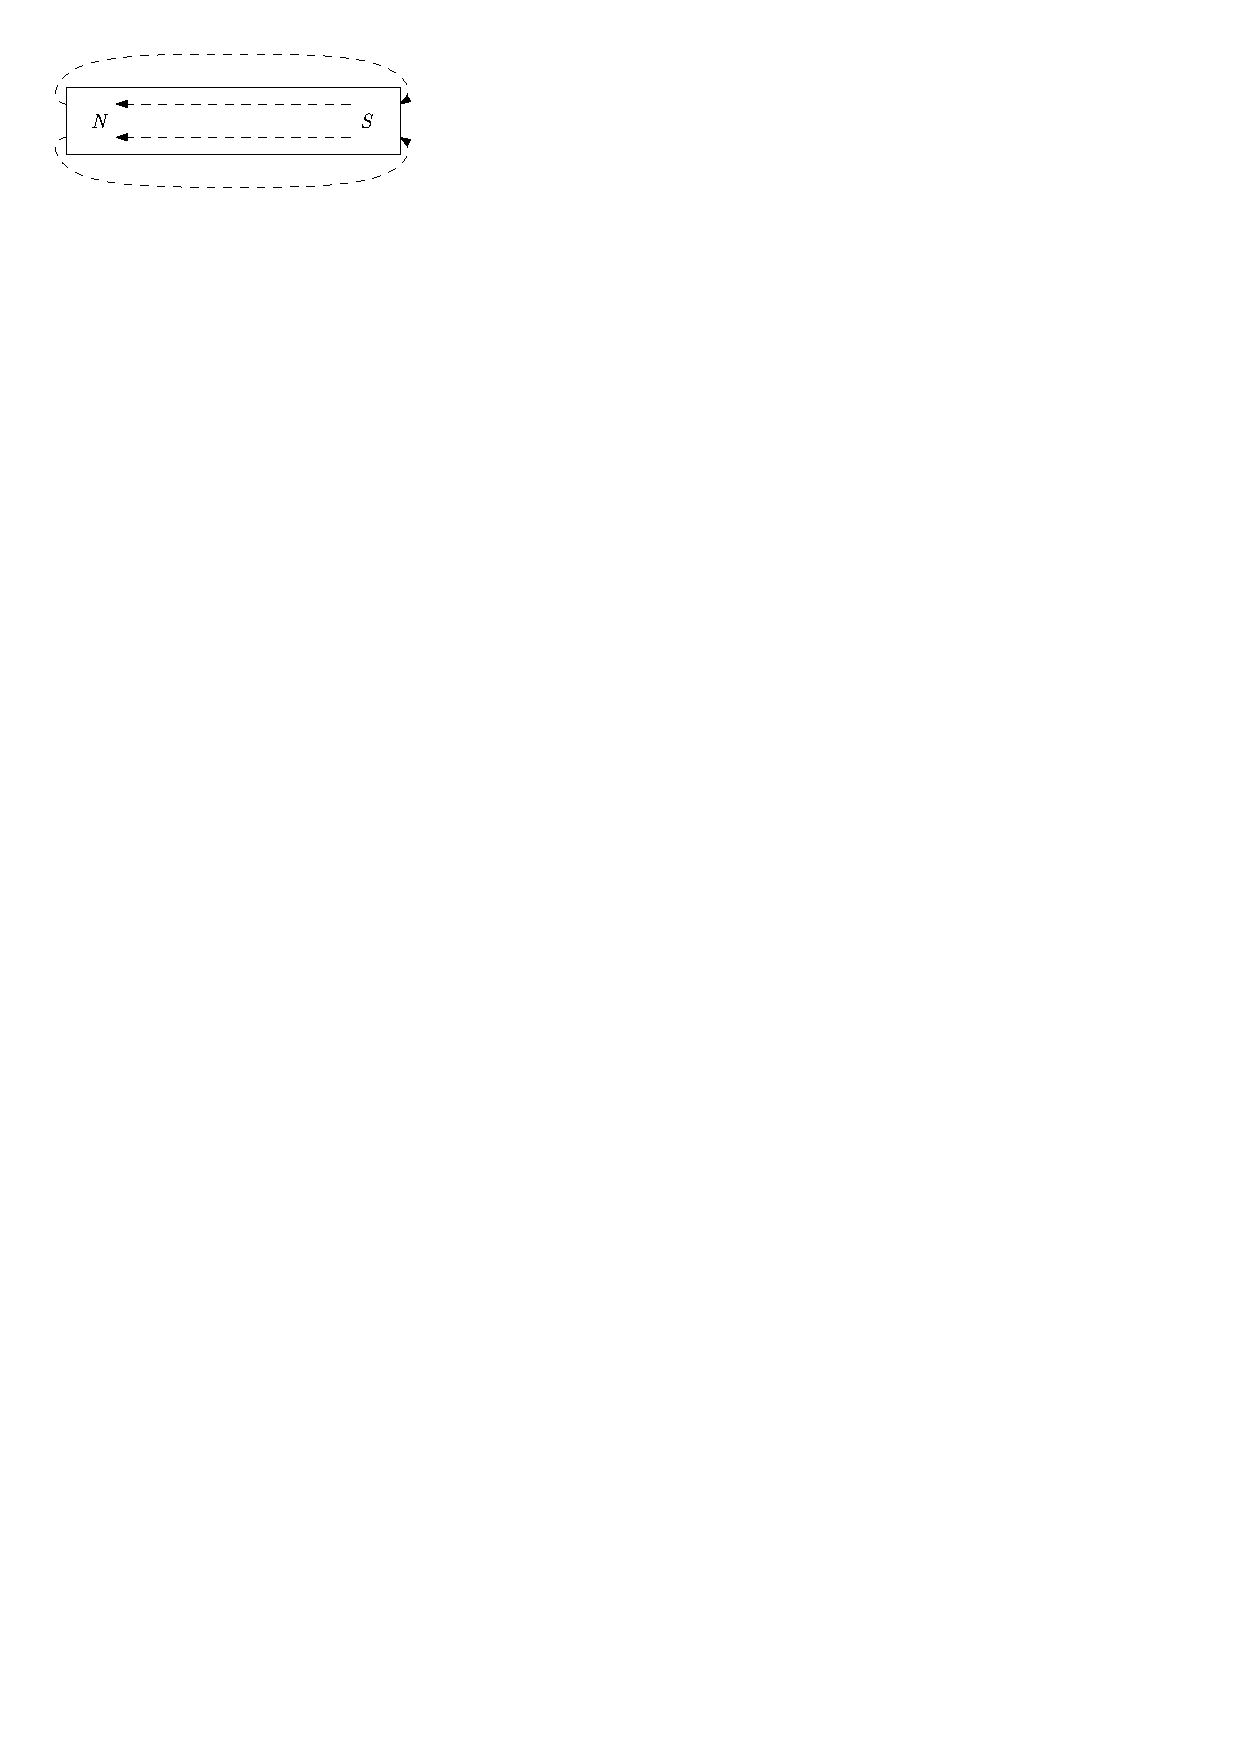
\includegraphics{figures/magnet-direction.pdf}
        \caption{The direction of flow from $N\rightarrow S$}
      \end{figure}
      \item magnetism is caused by moving charge
      \item \textbf{right hand rule}
      \begin{figure}[H]
        \centering
        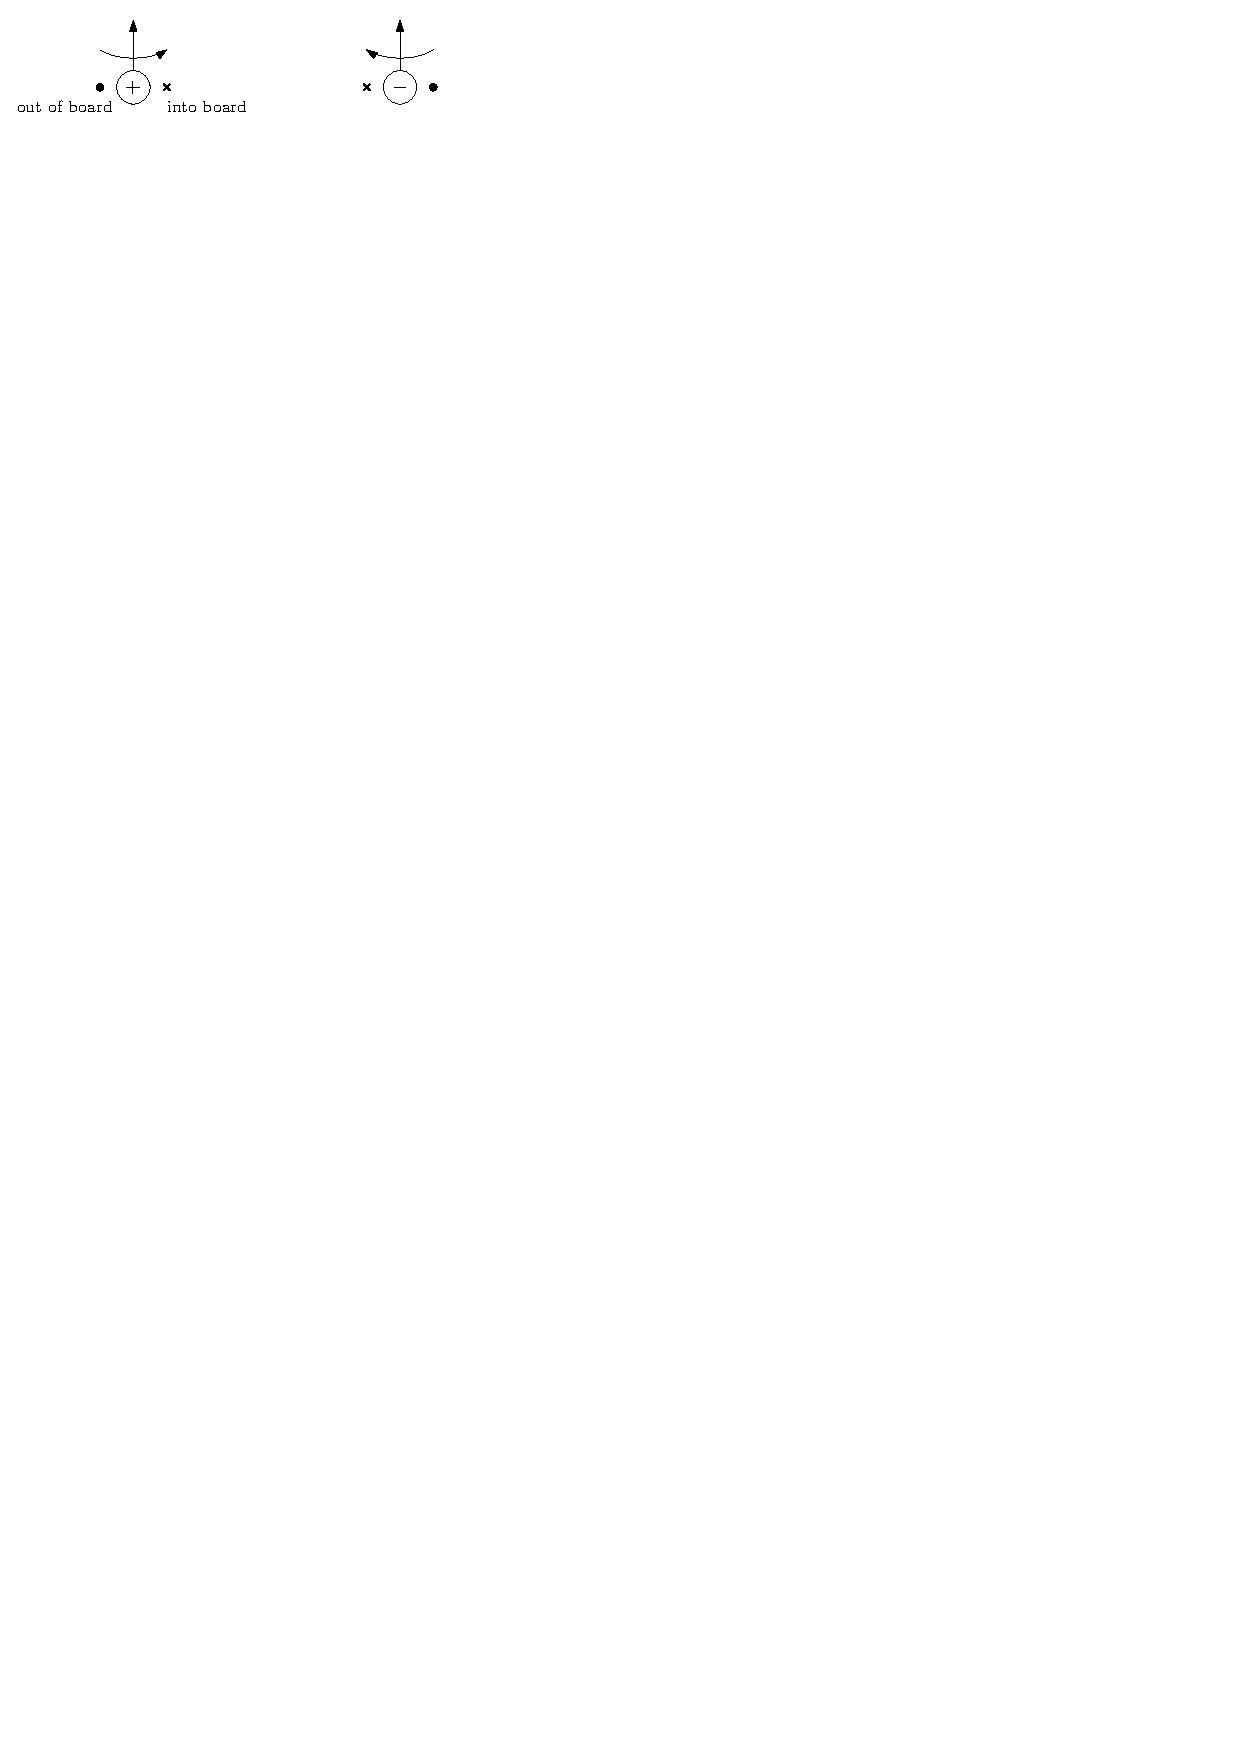
\includegraphics{figures/rhrule.pdf}
        \caption{How to determine direction using the right hand rule}
      \end{figure}
      \begin{figure}[H]
        \centering
        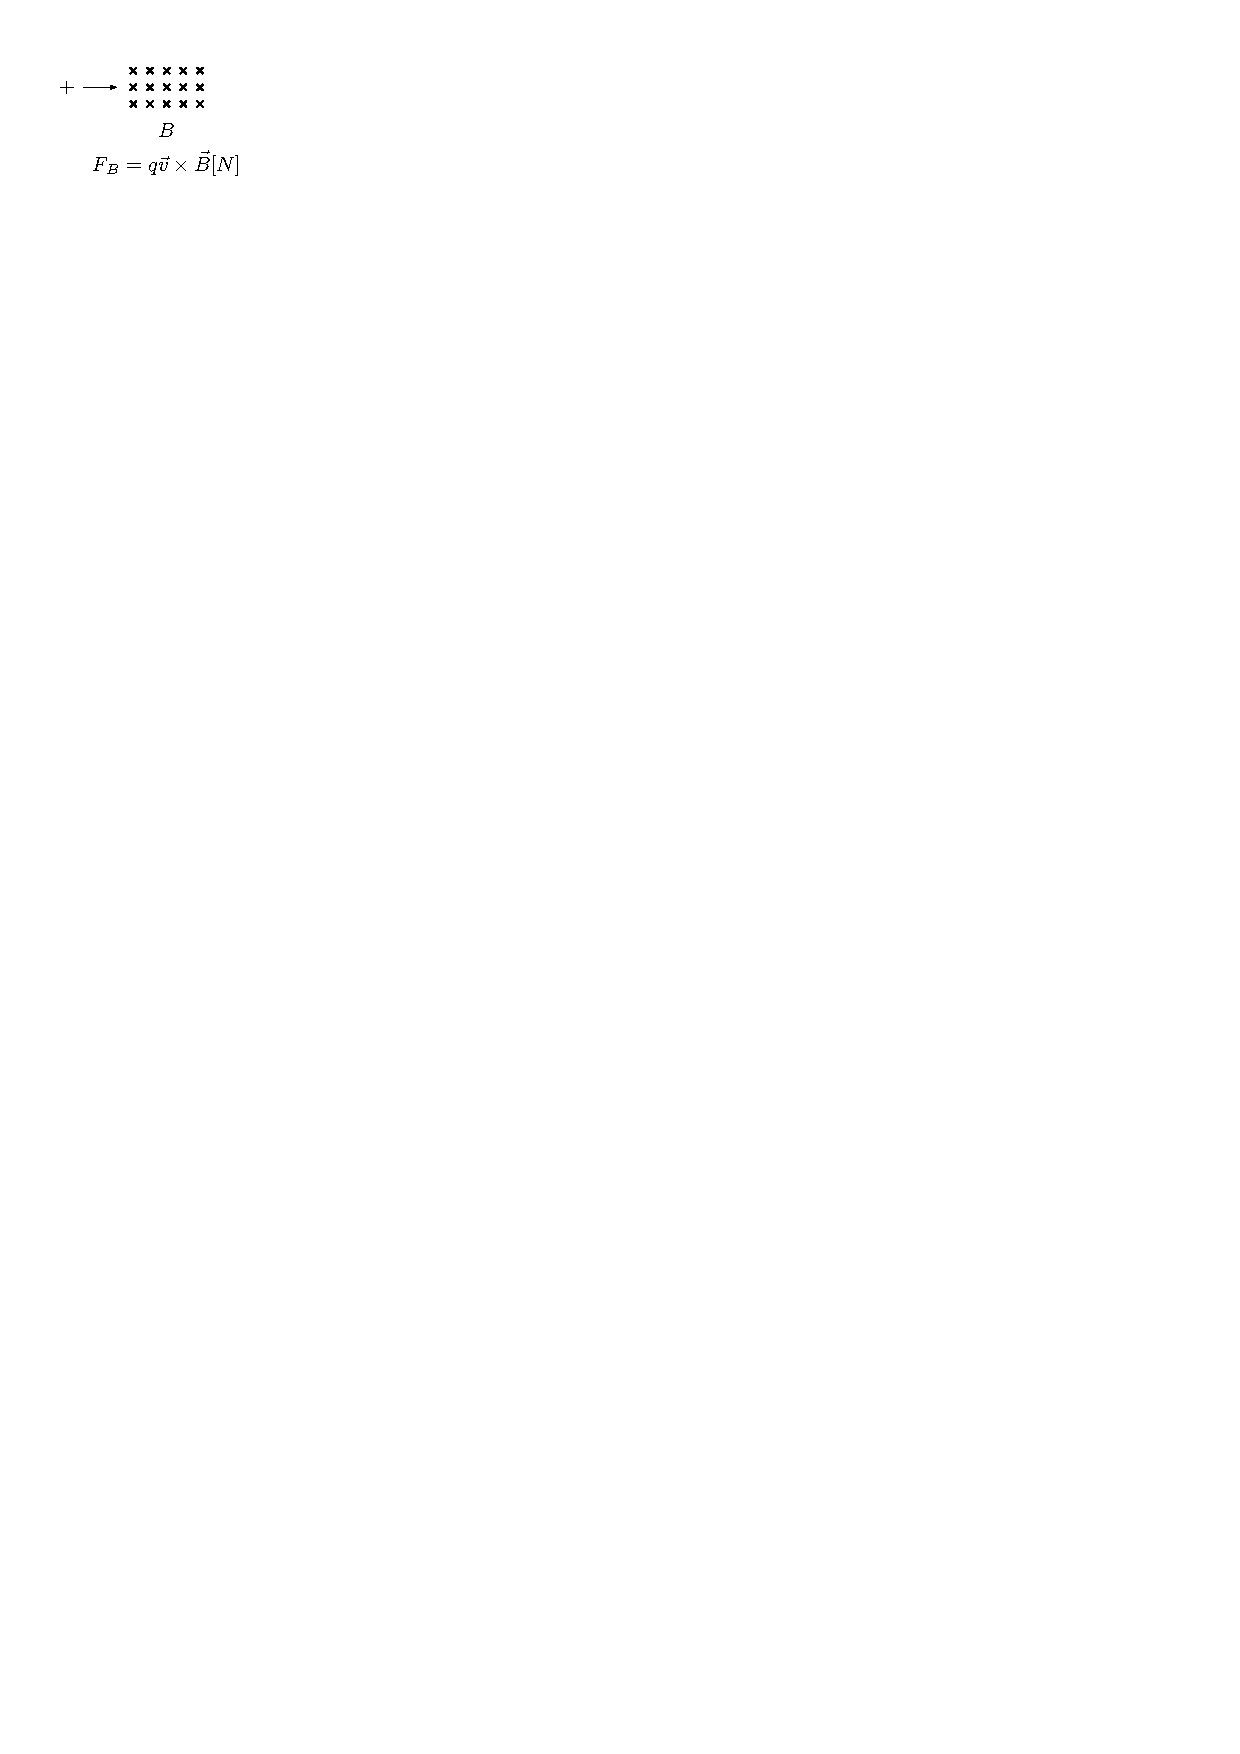
\includegraphics{figures/force-on-moving-charge.pdf}
        \caption{How to calculate force on a moving charge}
      \end{figure}
      \begin{figure}[H]
        \centering
        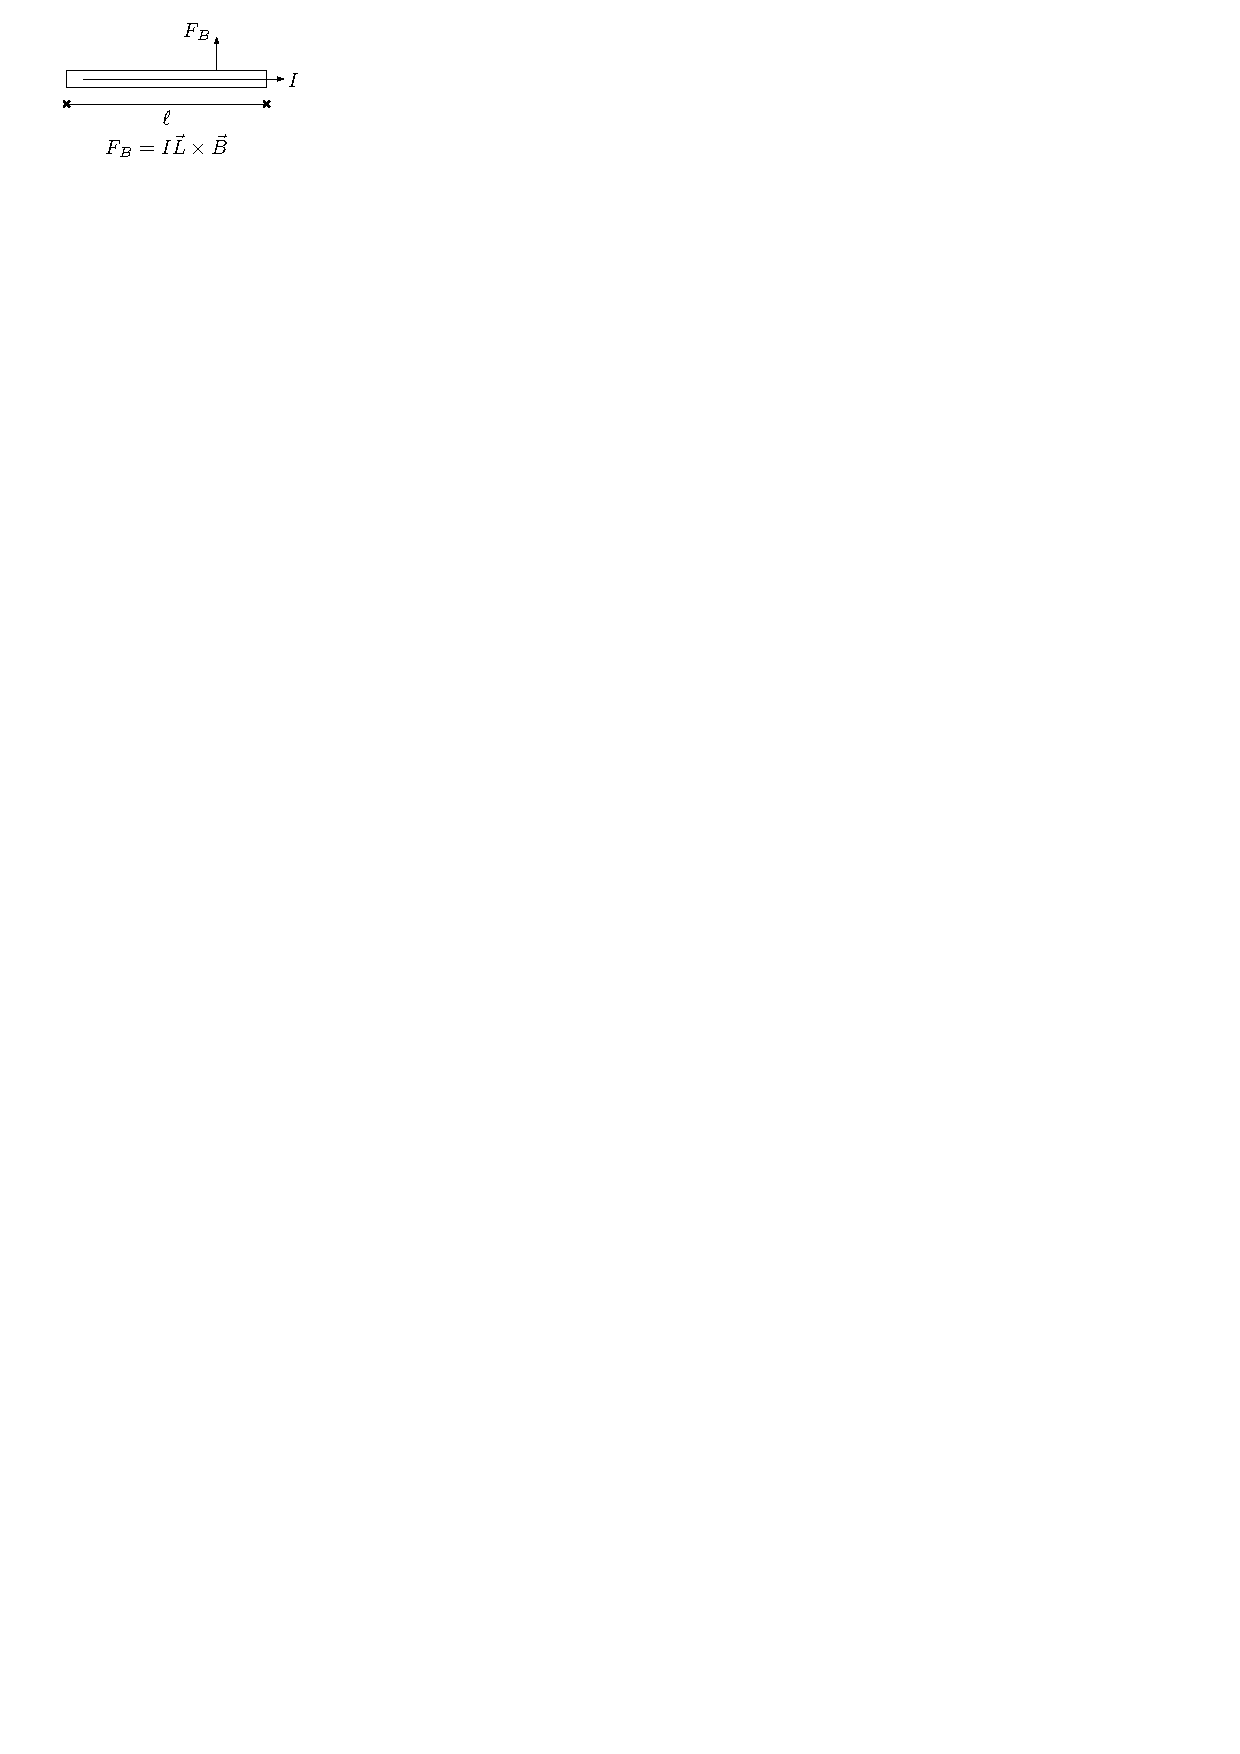
\includegraphics{figures/force-on-straight-wire.pdf}
        \caption{How to calculate force on a straight wire}
      \end{figure}
      \item \textbf{Biot-Savart Law}: an equation that describes the magnetic field in space
        \begin{itemize}
          \item \underline{Formula}:
            \begin{align*}
              |B| &= \frac{\mu_0}{4\pi}\cdot \frac{qV\sin(\theta)}{r^2}\\
               &=\frac{\mu_0}{4\pi}\cdot\frac{I\Delta S \times \hat{r}}{r^2}
            \end{align*}
            \begin{flushright}
              $\mu_0$: permeability of free space $\left[\frac{T\cdot m}{A}\right]$
            \end{flushright}
            \begin{figure}[H]
              \centering
              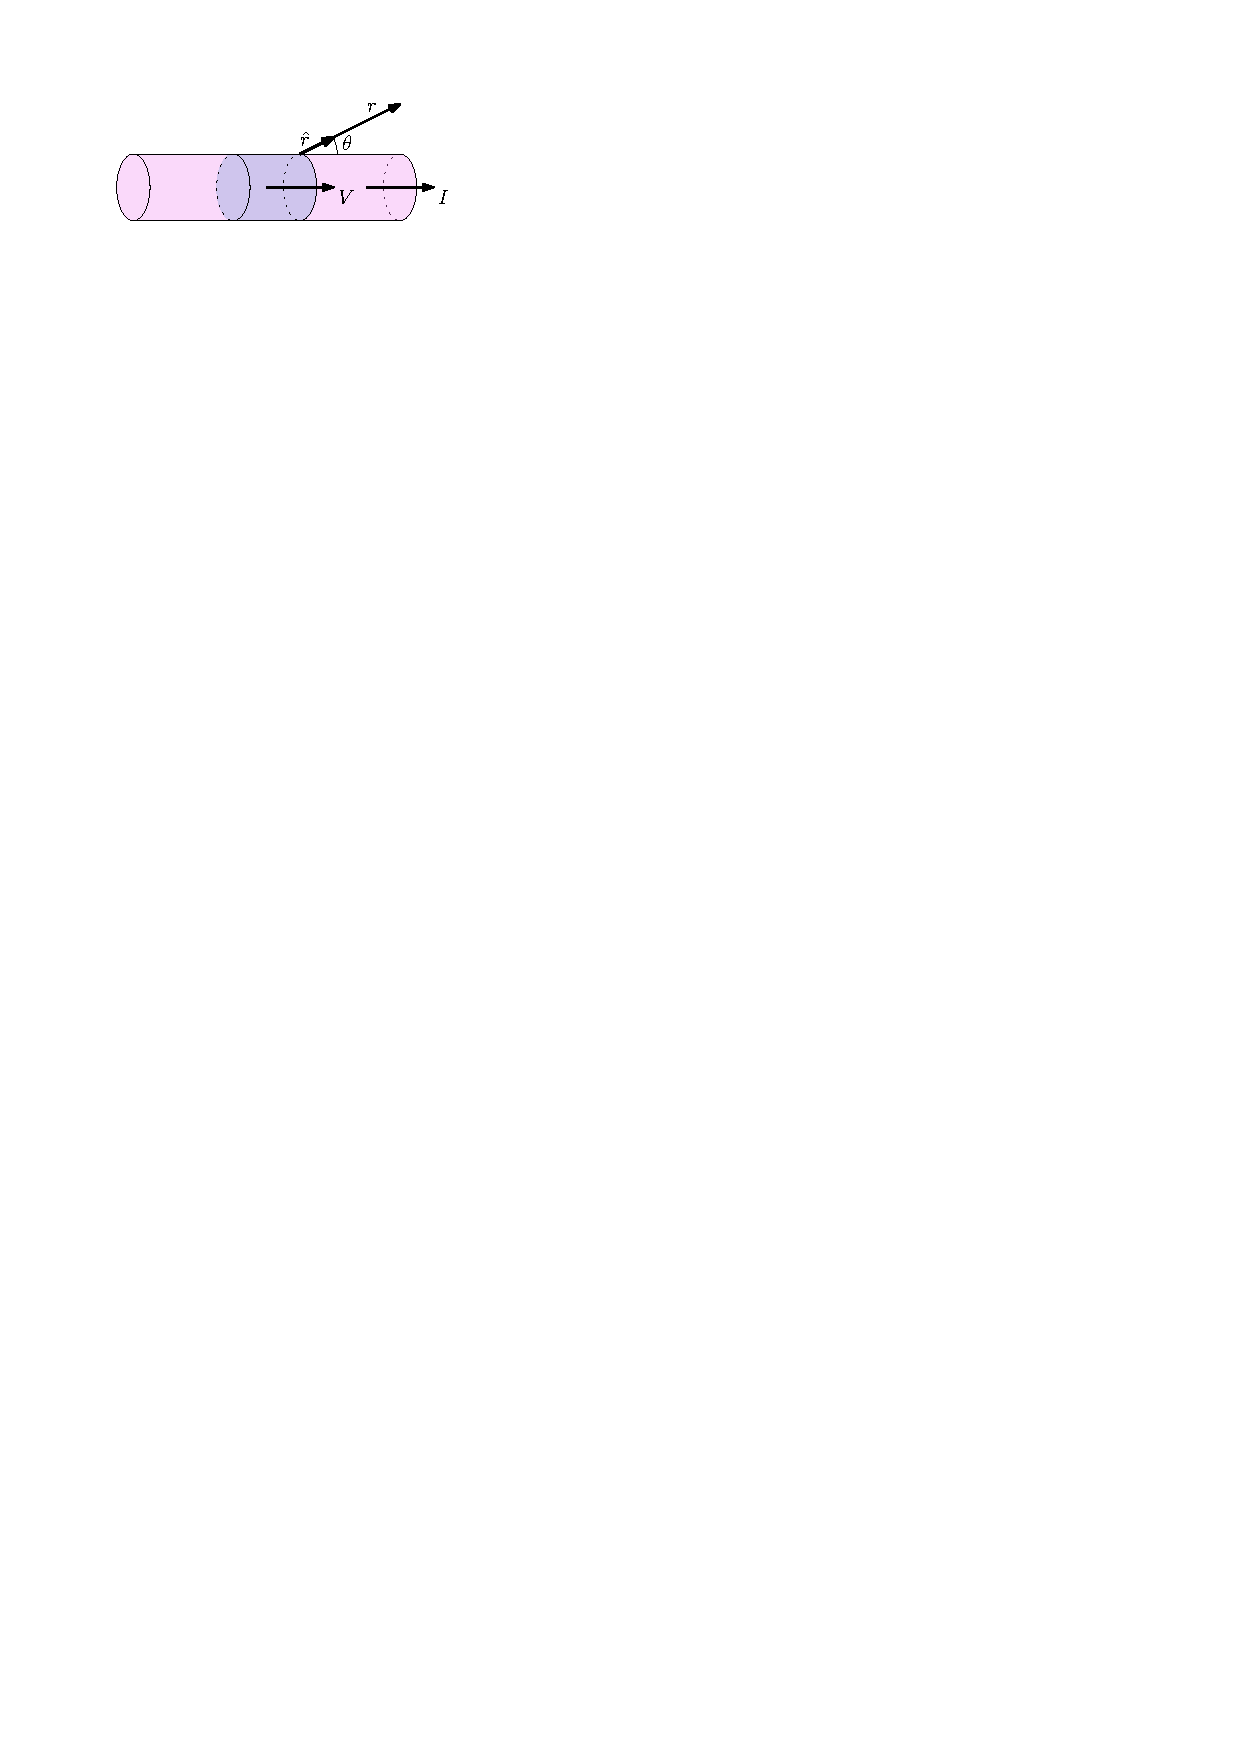
\includegraphics{figures/biot-savart.pdf}
              \caption{A diagram of the variables in Biot-Savart}
            \end{figure}
          \item \underline{Process} (to solve for $|B|$):
            \begin{enumerate}
              \item Draw a picture and choose coordinate axes
              \item Identify a point $P$
              \item Label ``$r$'', $\theta$ for at least two small sections $\Delta s$
              \item Use right hand rule to draw $B_i$ for each section
              \item Check for symmetry
              \item $B_{\mathrm{net}}=\sum B_i$
              \item Need algebraic expression for $B_x, B_y, B_z$
              \item Write $r$ and $\theta$ in terms of $x,y,z$
              \item Identify limits of integration
              \item Integrate
                \begin{figure}[H]
                  \centering
                  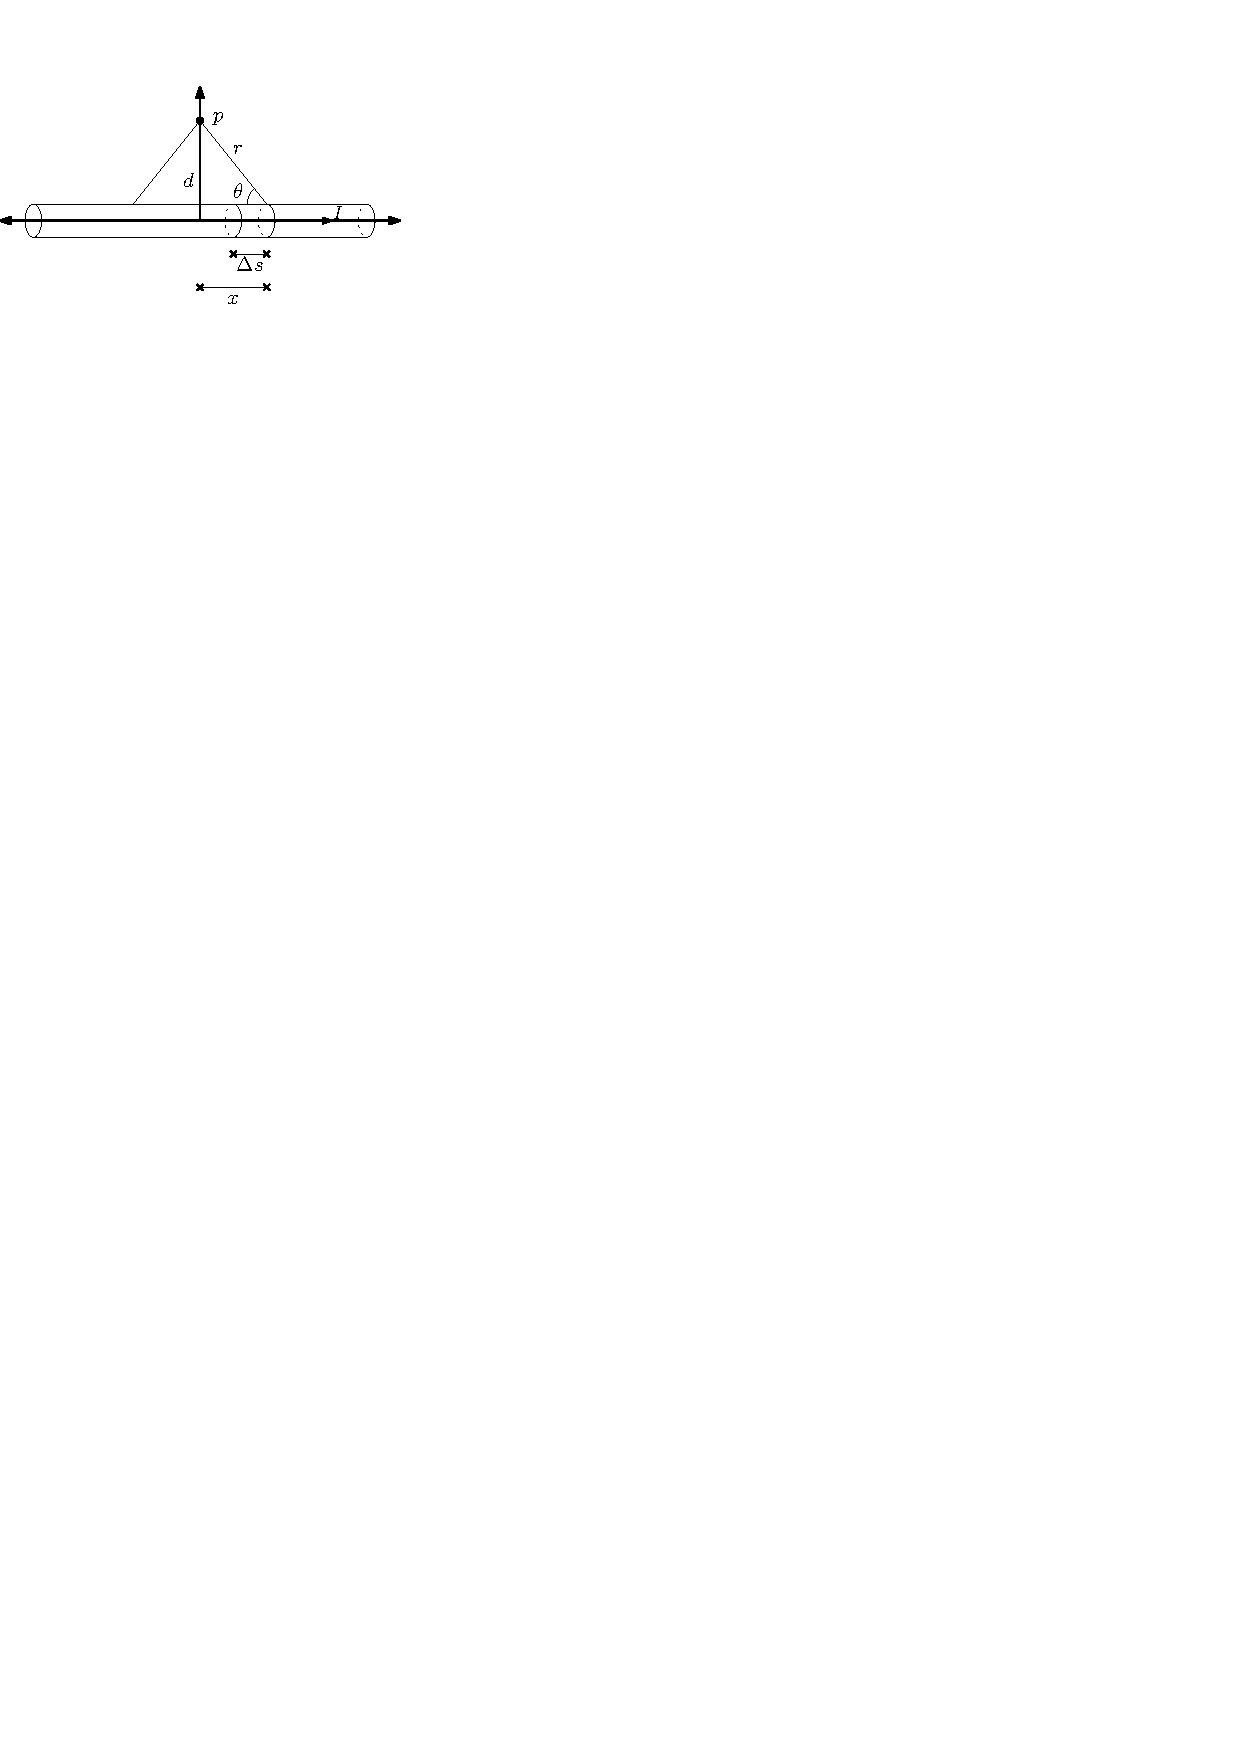
\includegraphics{figures/solving-biot-savart.pdf}
                  \caption{How to setup solving Biot-Savart for a straight wire}
                \end{figure}
                \begin{figure}[H]
                  \centering
                  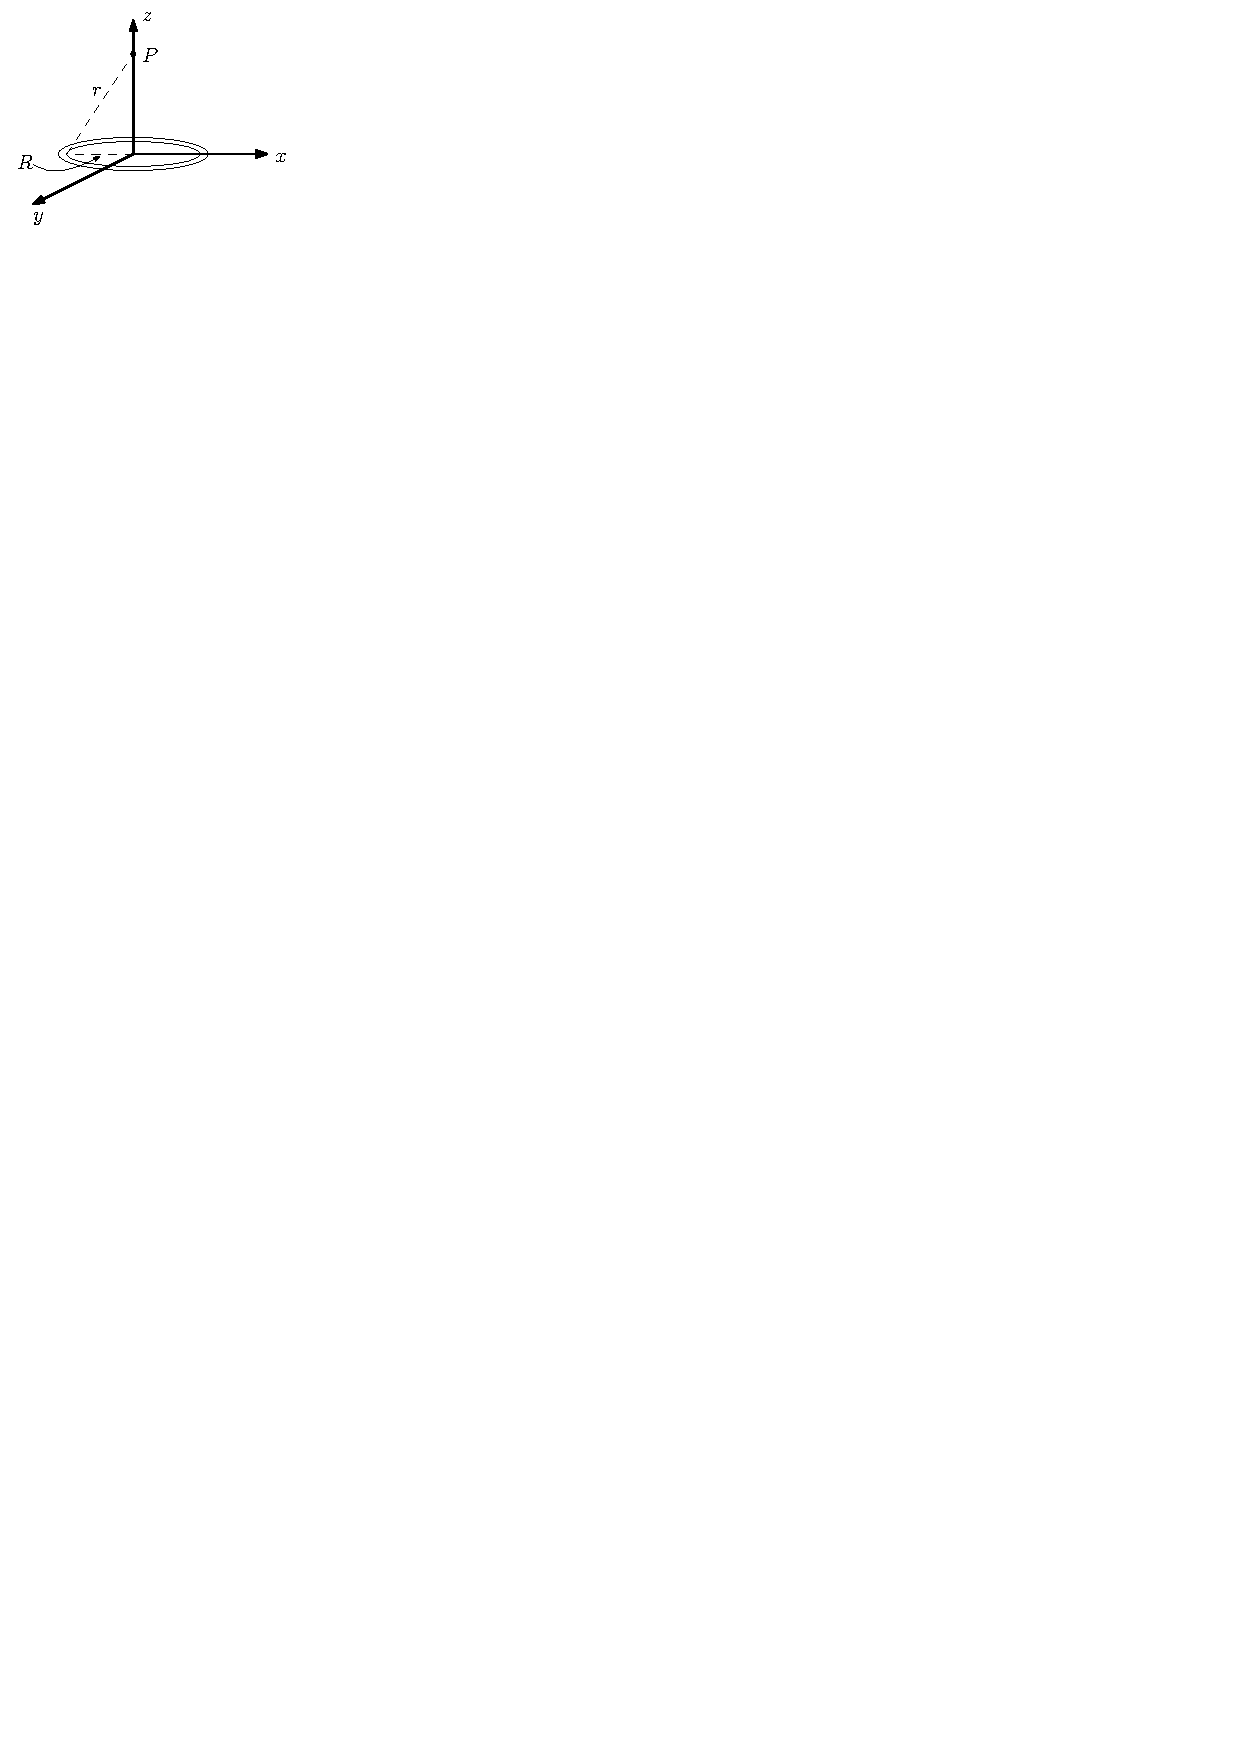
\includegraphics{figures/biot-savart-ring.pdf}
                  \caption{How to setup solving Biot-Savart for a ring}
                \end{figure}
            \end{enumerate}
        \end{itemize}
      \item \textbf{Ampere's Law}
        \begin{itemize}
          \item Ampere vs. Gauss
          \begin{itemize}
            \item Gauss: used to find $\vec{E}$ in \textit{highly symmetrical charge distribution}
              \begin{itemize}
                \item $\oint \vec{E}\cdot \dd A=\frac{Q_{\mathrm{enc}}}{\varepsilon_0}$
              \end{itemize}
            \item Ampere is the same principle
          \end{itemize} 
          \item only works when $\vec{B}$ is highly symmetric, i.e. $\vec{B}$ is the same magnitude at $r$ and is tangent to line $\dd \ell$
          \item \underline{Equation} 
            $$
              \oint_{\mathrm{c}} \vec{B}\cdot \dd \ell = \mu_0 I_{\mathrm{enc}}
            $$
            $$
              B_t = \frac{\mu_0 I_0}{2\pi r}
            $$
          \begin{figure}[H]
            \centering
            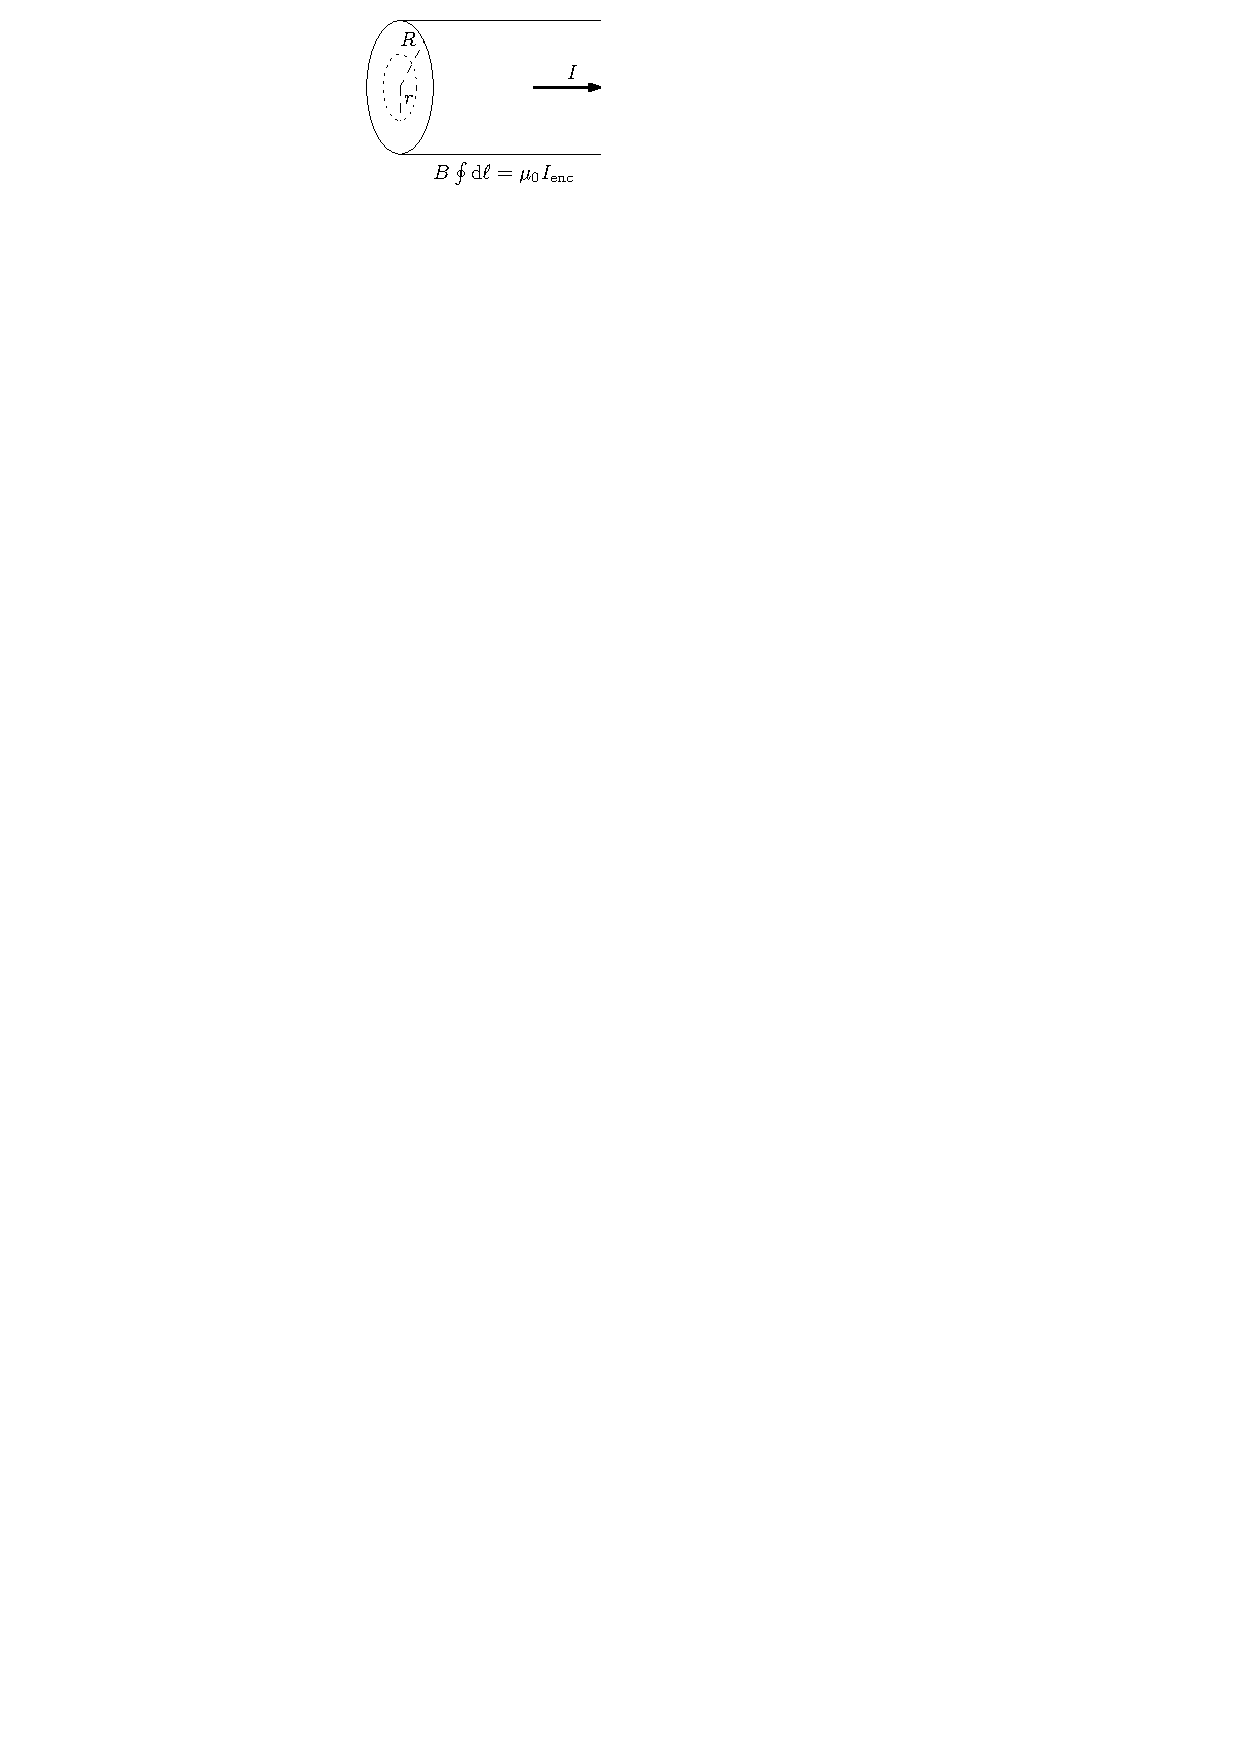
\includegraphics{figures/ampere1.pdf}
            \caption{Setting up Ampere's law for a wire}
          \end{figure}
          \begin{figure}[H]
            \centering
            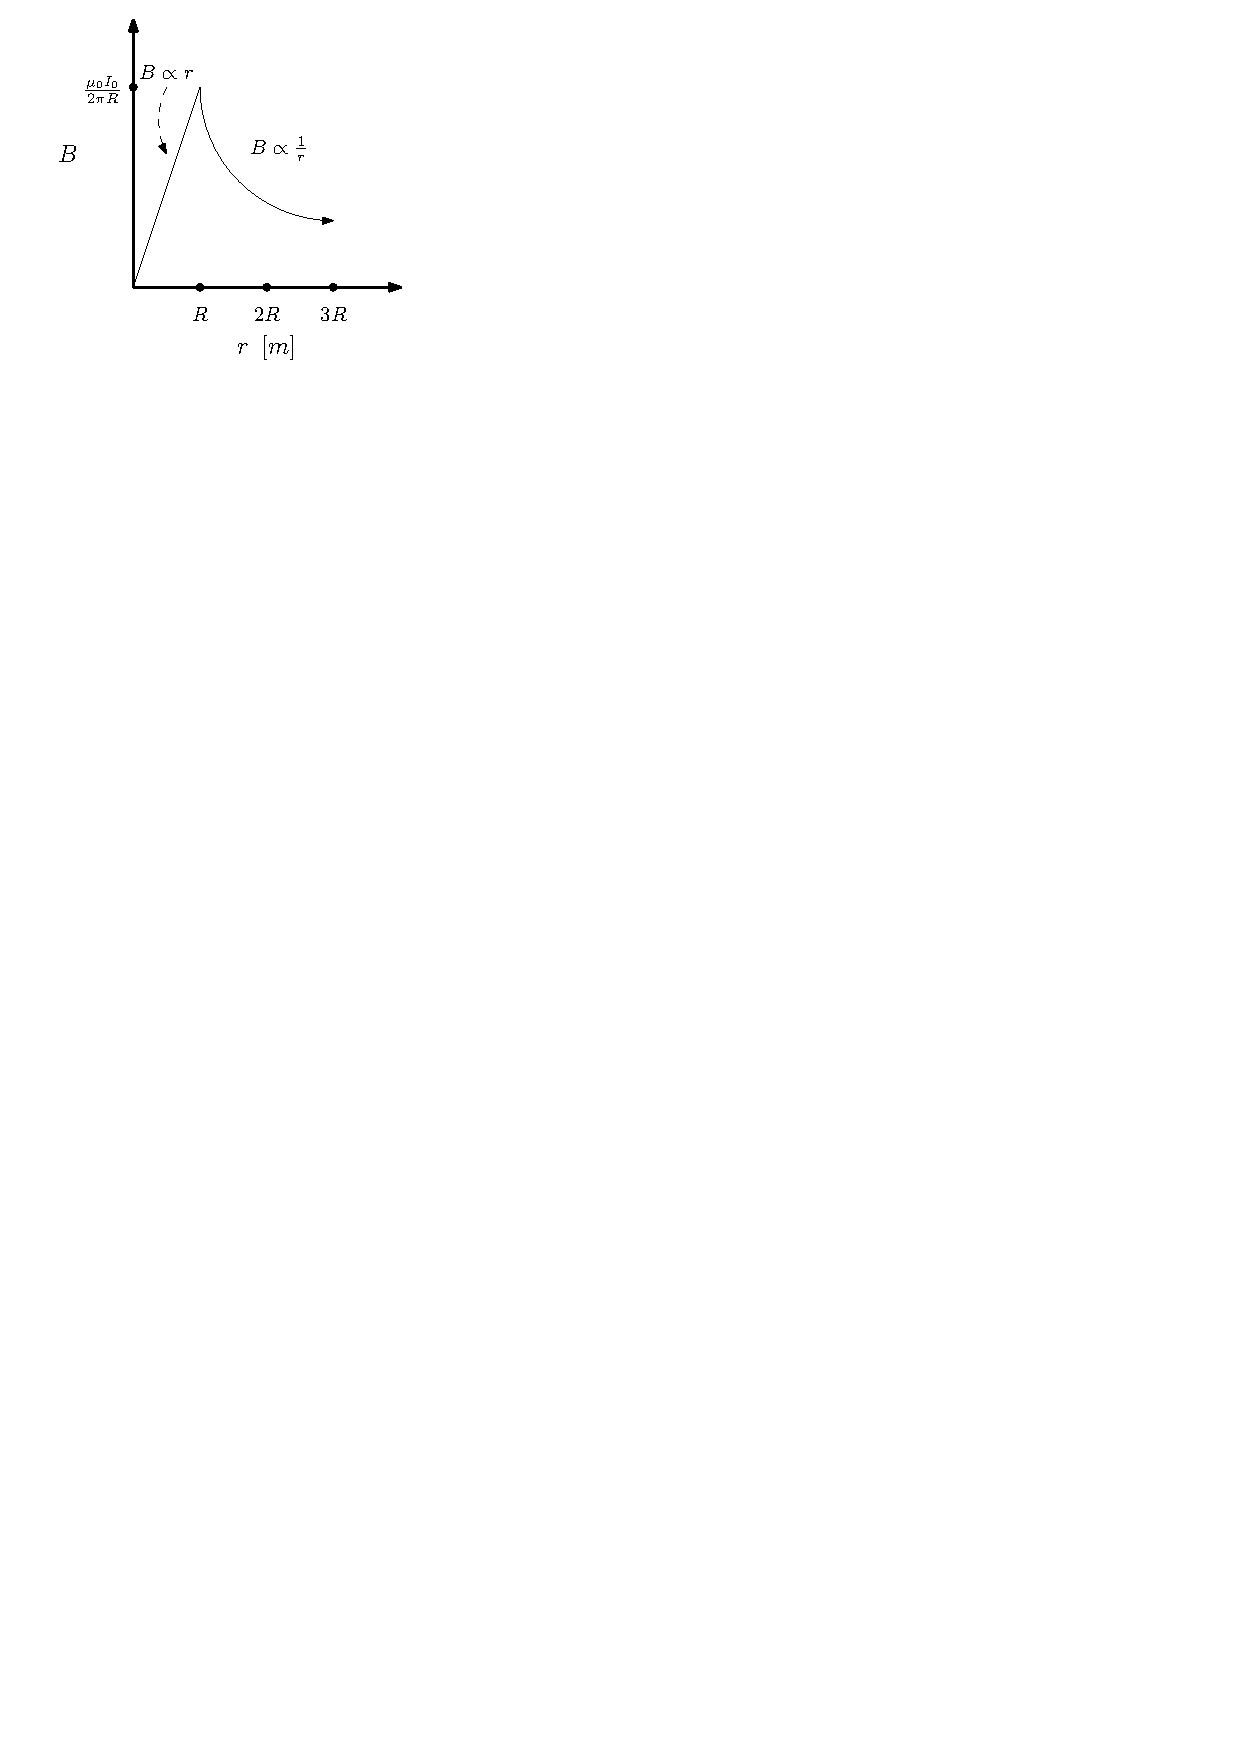
\includegraphics{figures/BvsR.pdf}
            \caption{$B$ vs. $r$ in a constant-current circuit (wire)}
          \end{figure}
          \item \underline{Solving}:
            \begin{align*}
              B_t \oint\dd l & =\mu_0 I_{\mathrm{enc}}\\2
              B_t &= \frac{\mu_0}{2\pi r} \cdot I_0 \cdot \frac{r^2}{R^2}\\
               & = \frac{\mu_0}{2\pi \cancel{r}} \cdot I_0 \cdot \frac{r^{\cancel{2}}}{R^2}
            \end{align*}
          \begin{figure}[H]
            \centering
            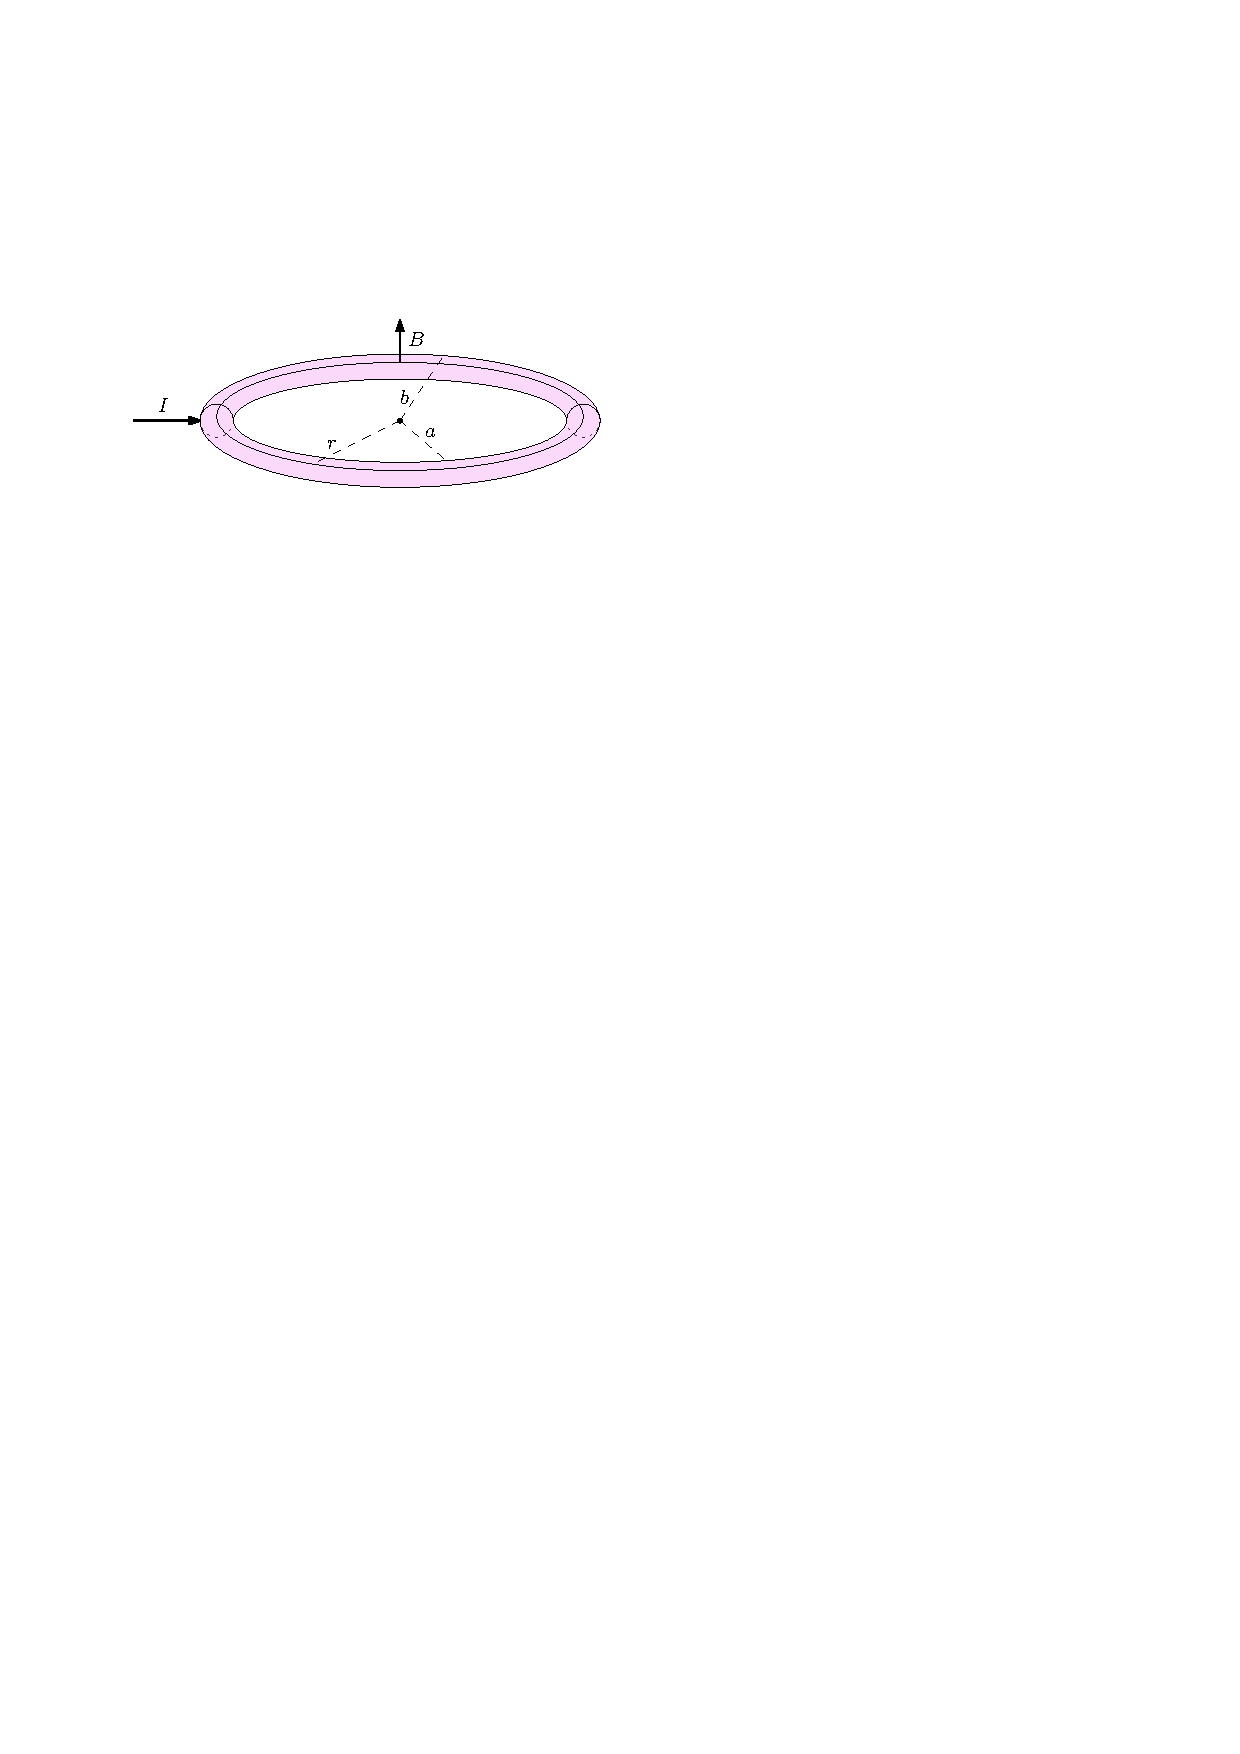
\includegraphics{figures/ampere2.pdf}
            \caption{Setting up Ampere's law for a toroid}
          \end{figure}
          \begin{figure}[H]
            \centering
            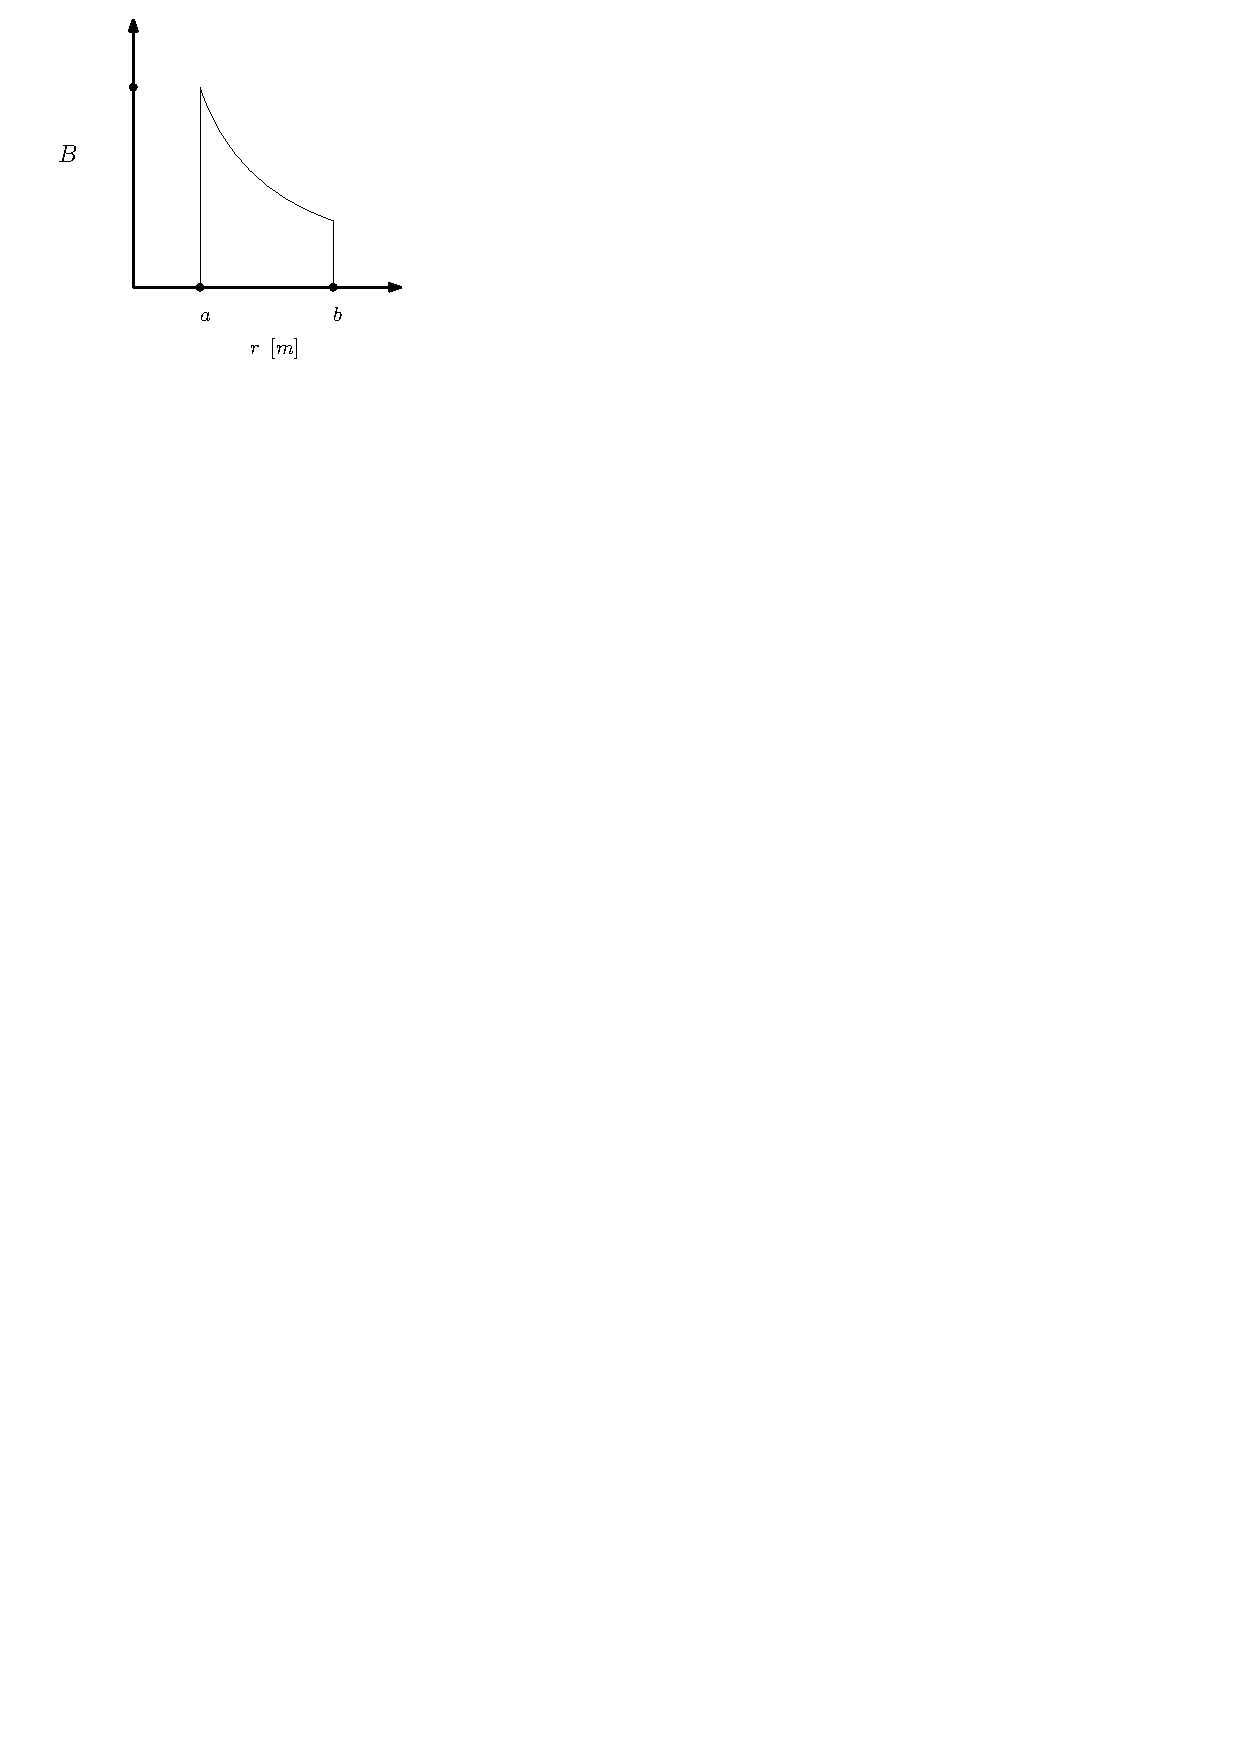
\includegraphics{figures/BvsR2.pdf}
            \caption{$B$ vs. $r$ in a constant-current circuit (toroid)}
          \end{figure}
        \end{itemize}
      \item \textbf{magnetic flux ($\Phi_m$)}: the amount of magnetic field that passes through a coil
        $$\Phi_m = \vec{B}\cdot\vec{A} = |B||A|\cos(\theta)$$
    \end{itemize}
  \section{Induction}
    \begin{itemize}
      \item \textbf{electromagnetic induction}: moving magnet creating an electric field
      \item $I$ induced only occurs when $\vec{B}$ is changing within the coil
        \begin{itemize}
          \item Keep coil stationary and change $\vec{B}$
          \item Keep $B$ stationary and change coil
            \begin{itemize}
              \item Change either area or orientation of the coil
            \end{itemize} 
        \end{itemize}
      \begin{figure}[H]
        \centering
        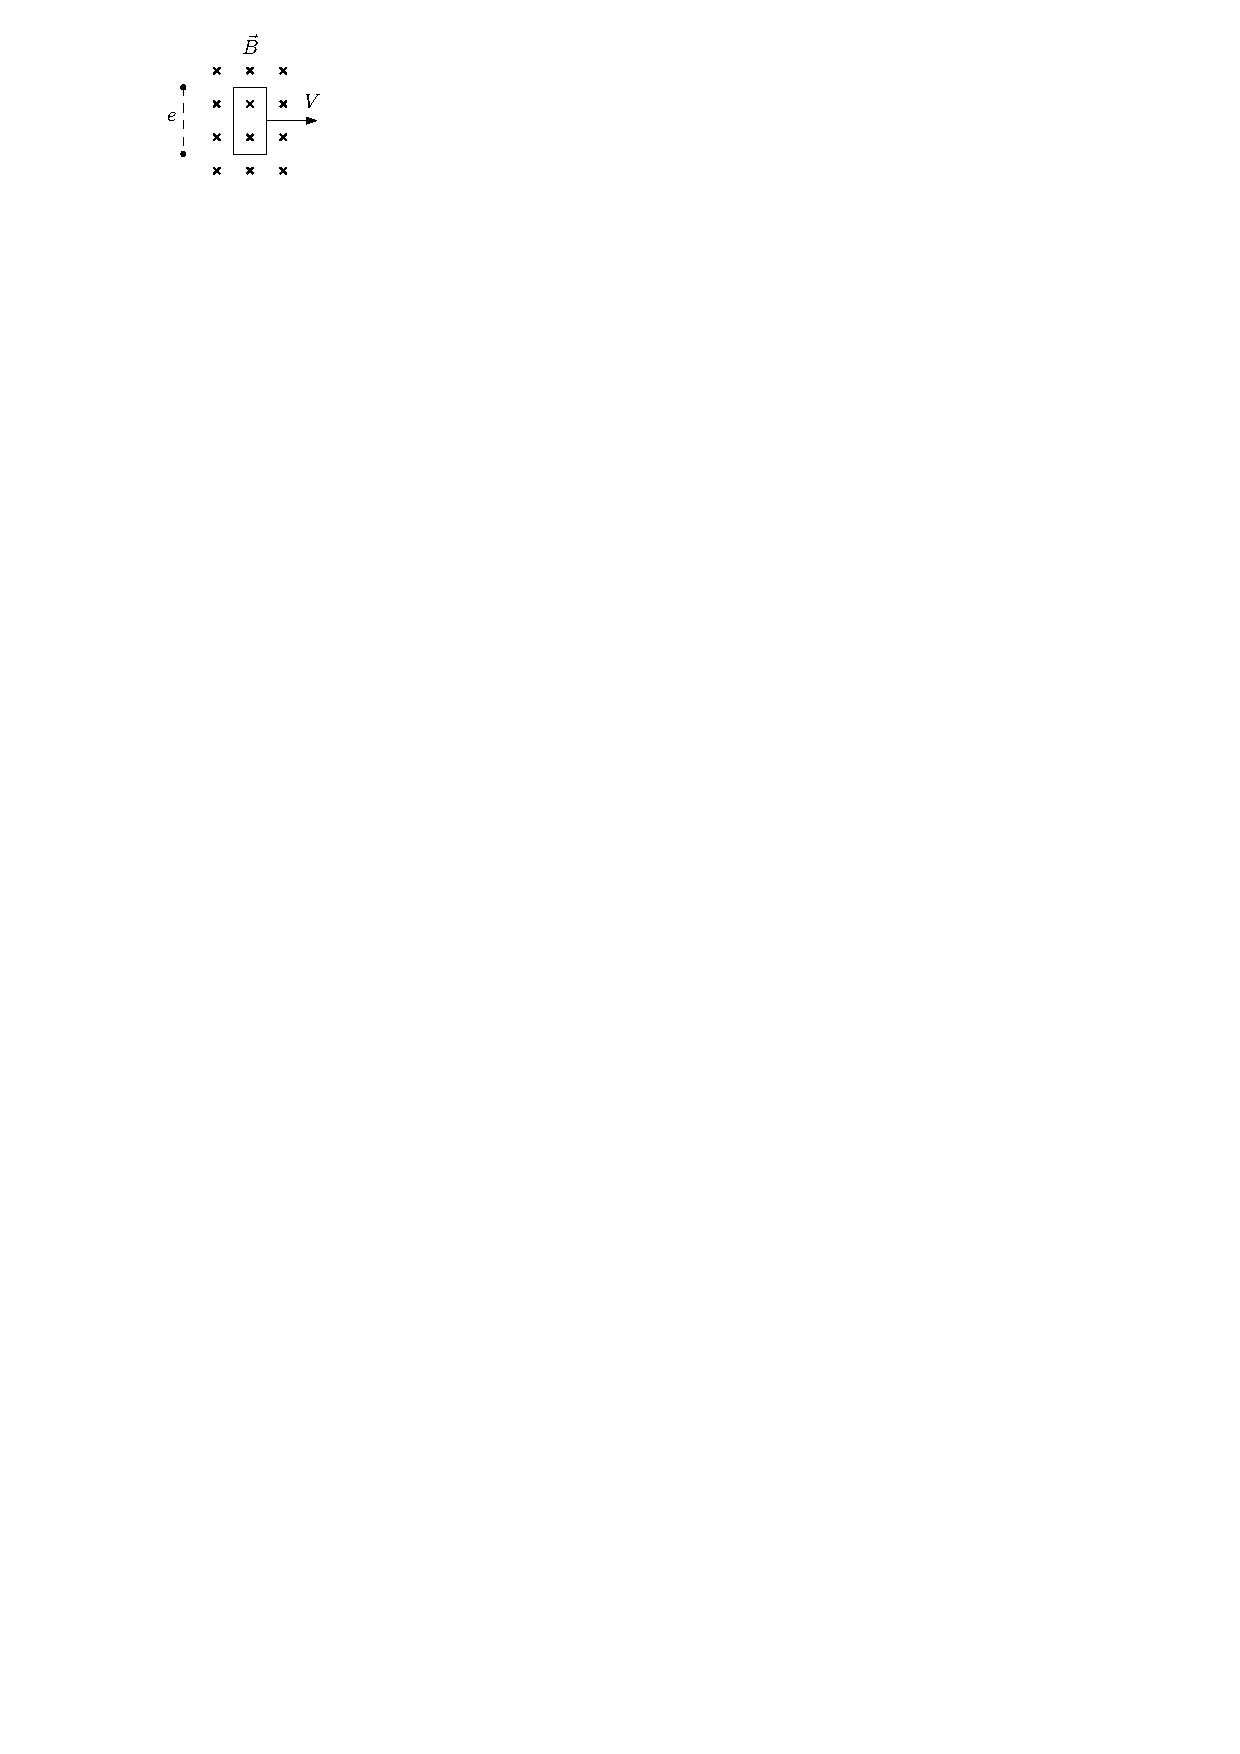
\includegraphics{figures/faraday1.pdf}
        \caption{Motional EMF}
      \end{figure}
      \item \underline{Solving} (to find EMF):
      \begin{align*}
        \sum F &= 0\\
        F_B & = F_E\\
        \cancel{q} vB & = \cancel{q}E\\
        E_{\mathrm{inside}} &= vB
      \end{align*}
      Then to find EMF:
      \begin{align*}
        \text{EMF} & =\Delta V\\
        \Delta V & = V_f-V_i=-\int E\cdot \dd \ell\\
        \text{EMF} & = - \int E_{\mathrm{inside}} \cdot \dd \ell\\ 
         & = -(-Bv)\ell\\
        \varepsilon & = Bv\ell
      \end{align*}
      \begin{figure}[H]
        \centering
        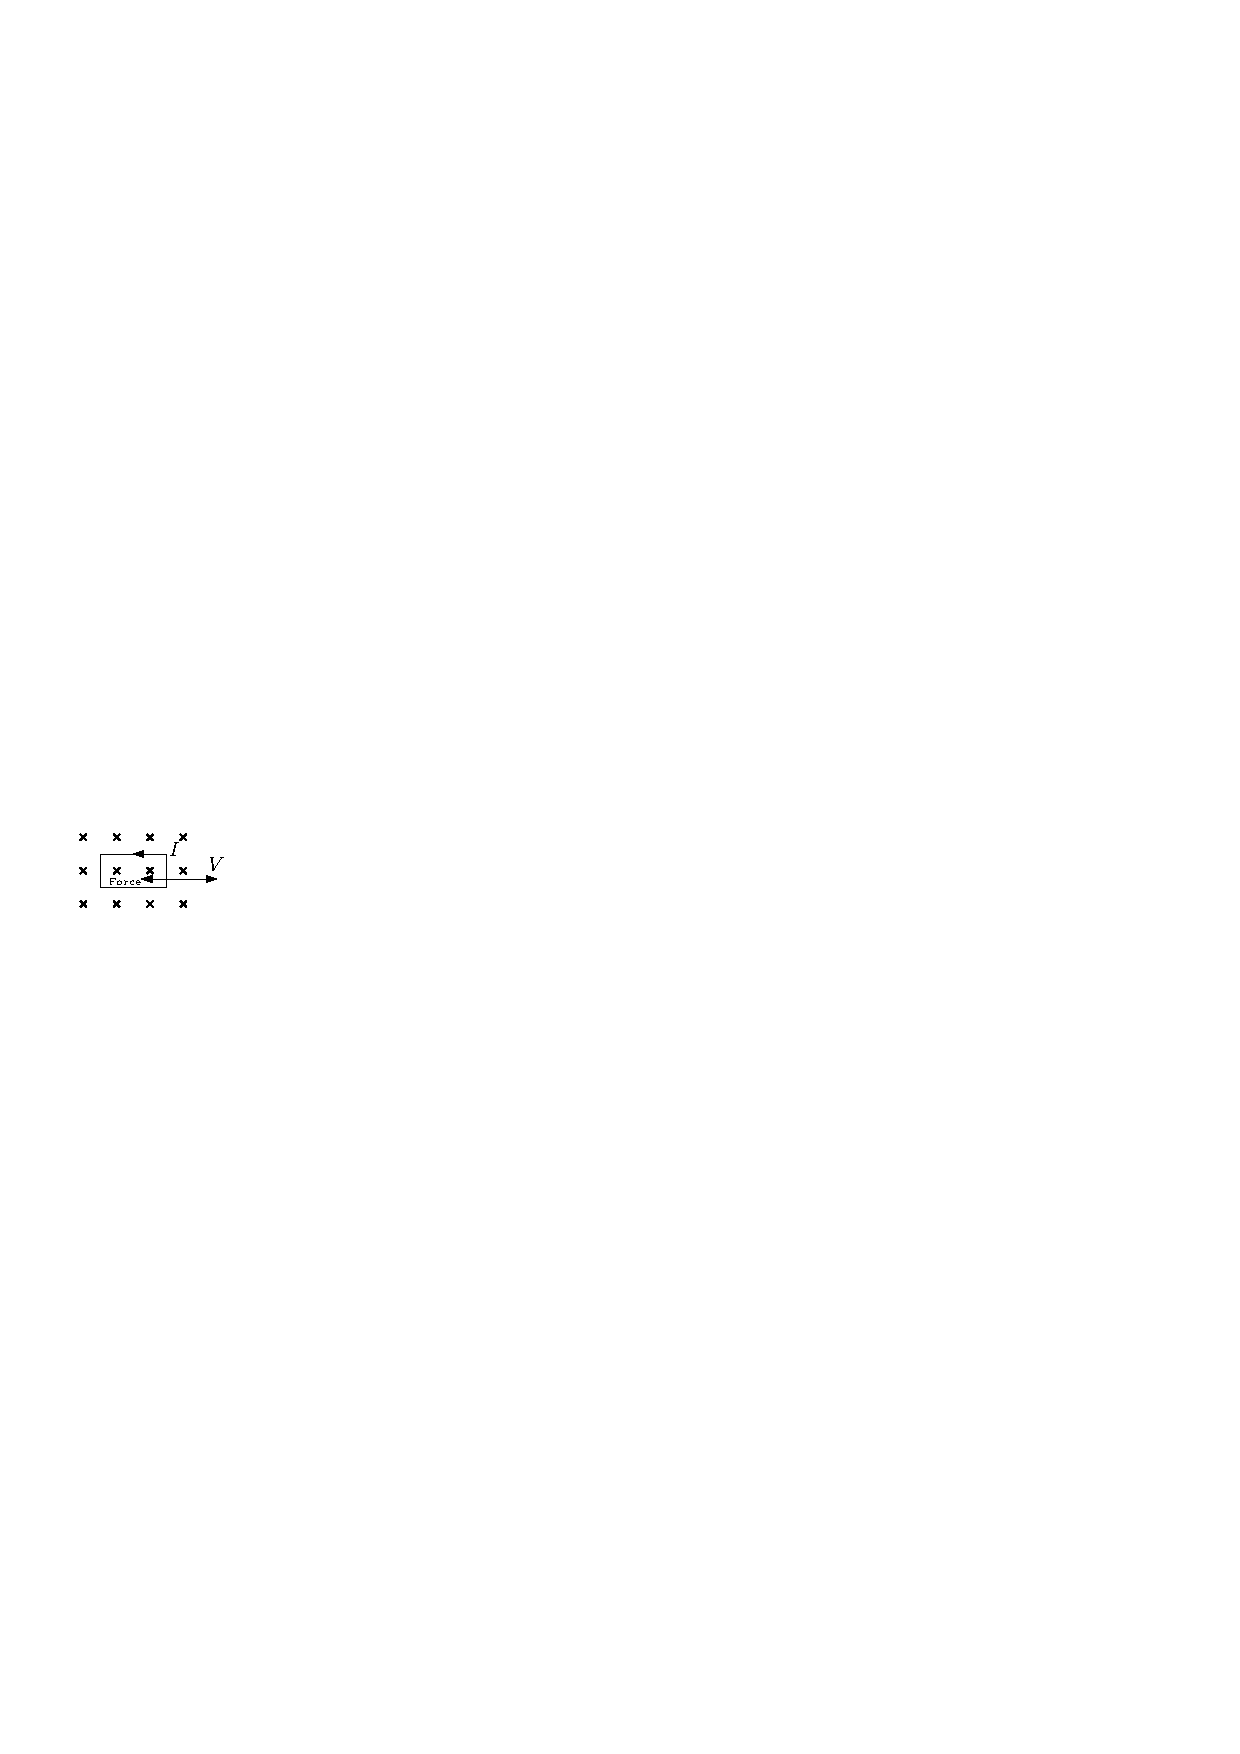
\includegraphics{figures/faraday2.pdf}
        \caption{Loop in magnetic field}
      \end{figure}
      \item \textbf{loop in magnetic field}
        \begin{itemize}
          \item drag force is opposite the velocity
          \item due to $B$ acting on $I$ induced
          \item \underline{Solving} (for $I$ induced):
            \begin{align*}
              I_{\mathrm{induced}} &= \frac{V}{R}\\
               & = \frac{Bv\ell}{R}
            \end{align*}
        \end{itemize} 
      \item \textbf{Lenz's Law}
        \begin{itemize}
          \item Induced current creates a magnetic field that opposes the change in $B$
        \end{itemize} 
      \item \textbf{Faraday's Law}
        \begin{itemize}
          \item \underline{Formula}:
            $$
            \varepsilon = \left|\frac{\dd \Phi_m}{\dd t}\right|
            $$
          \item $\varepsilon_{\mathrm{induced}}$ is the rate of change of magnetic flux in the coil
          \begin{figure}[H]
            \centering
            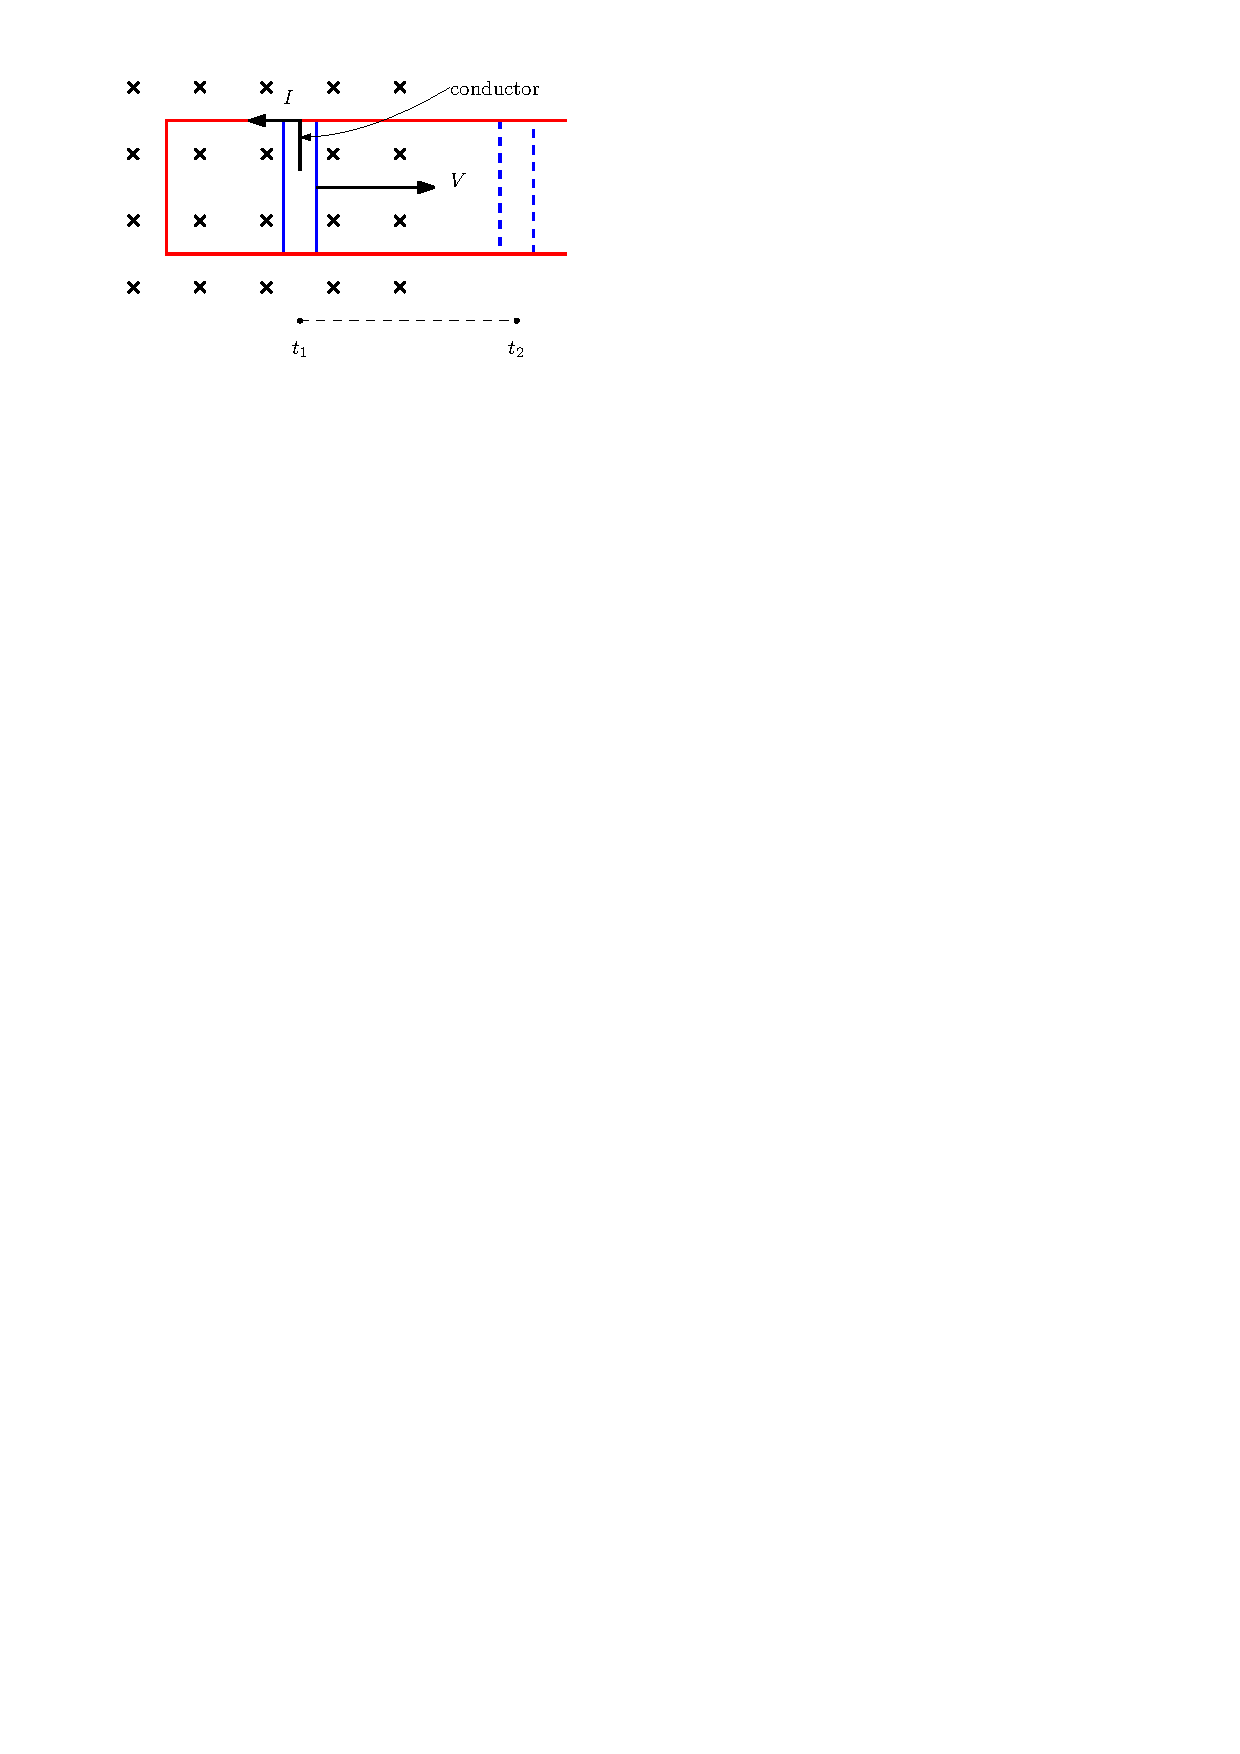
\includegraphics{figures/faraday3.pdf}
            \caption{The change in area}
          \end{figure}
          \item \underline{Solving}:
          \begin{align*}
            \varepsilon & = \left| \frac{\dd\Phi_m}{\dd t} \right|\\
             & = \frac{\dd B\ell x}{\dd t} & \Rightarrow \frac{\dd x}{\dd t} = v\\
             & = B\ell v
          \end{align*}
        \end{itemize} 
      \end{itemize}
    \section{Circuits}
      \begin{figure}[H]
        \centering
        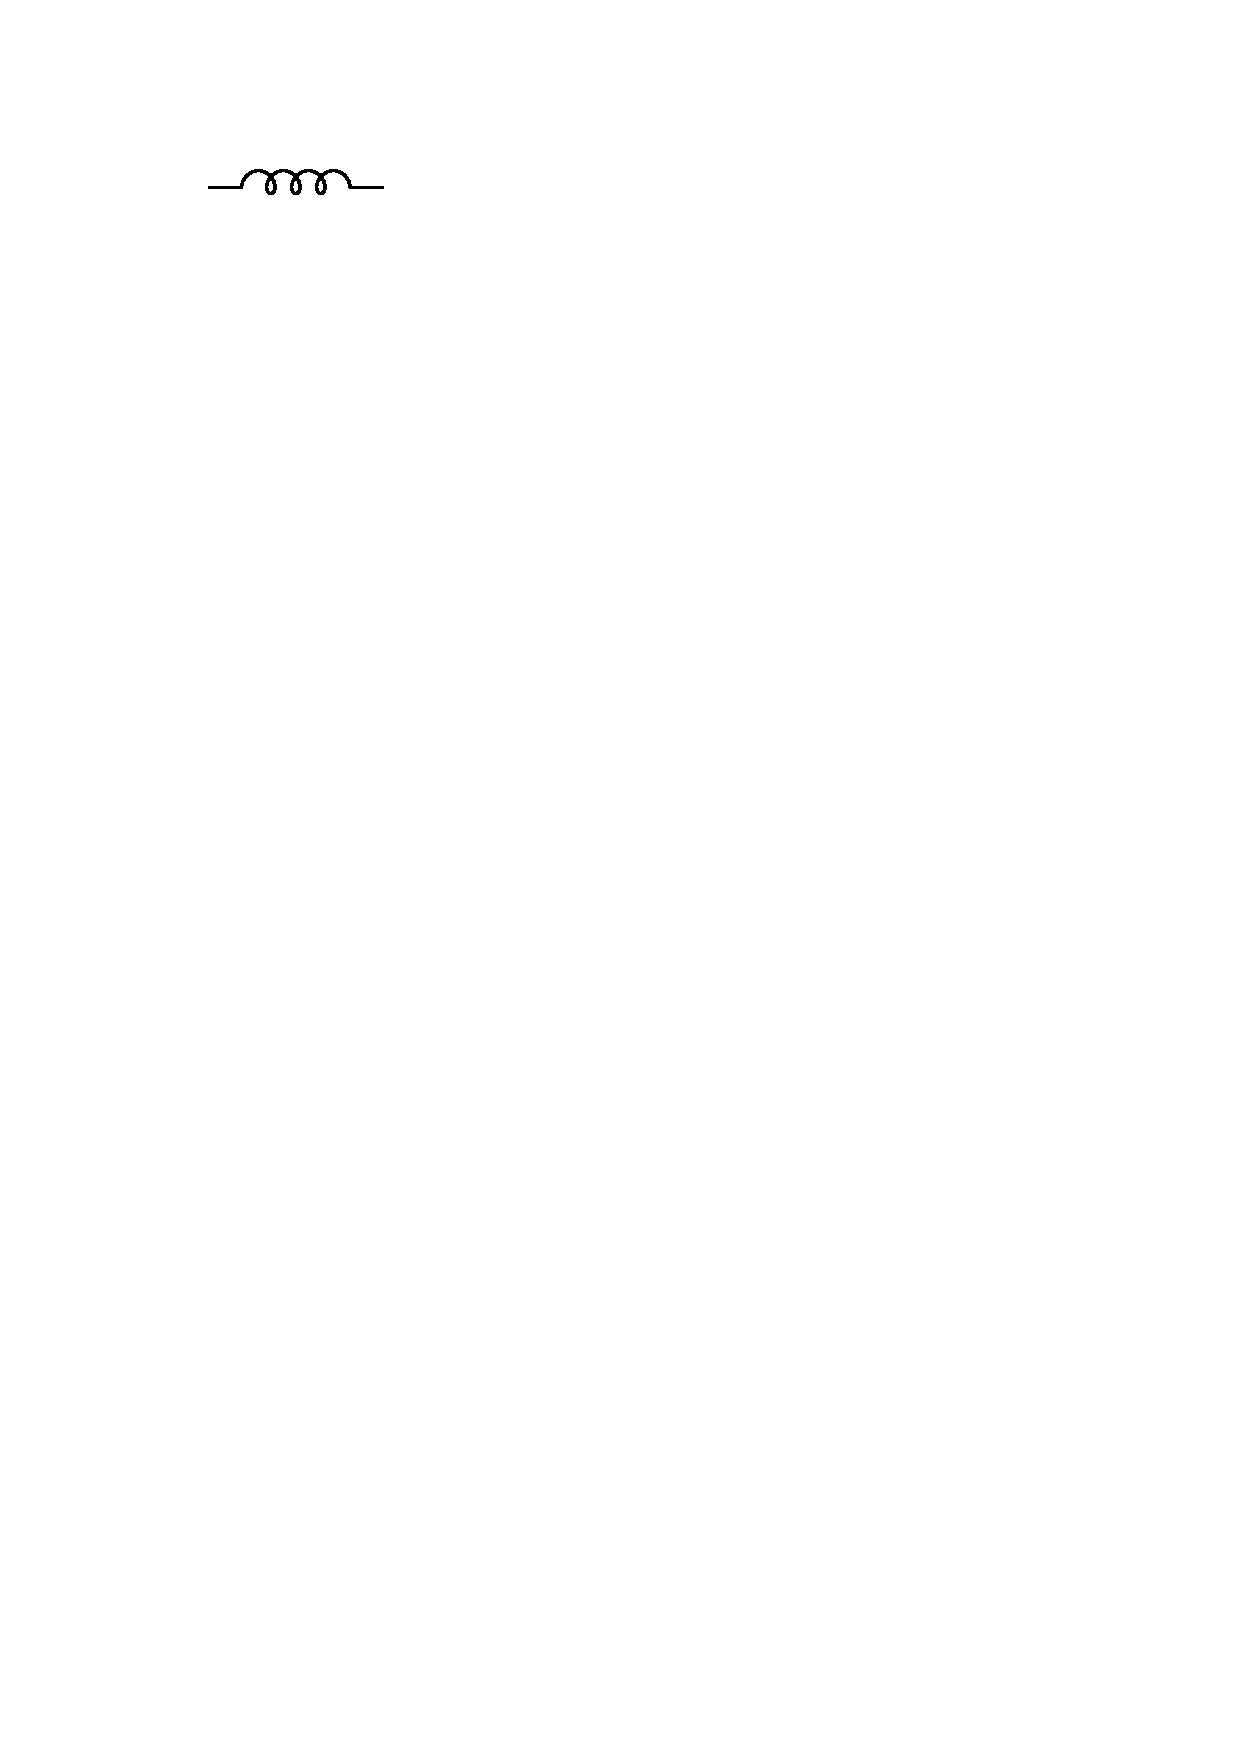
\includegraphics{figures/inductor.pdf}
        \caption{The circuit symbol for an inductor}
      \end{figure}
      \begin{itemize}
        \item \textbf{inductor}: slows down or resists a change in current
          \begin{itemize}
            \item has a unifrom magnetic field
          \end{itemize} 
        \item \textbf{inductance ($L\enspace[H]=\frac{\mathrm{Wb}}{\mathrm{Amp.}}$)}: the ratio of flux to current induced
          \begin{itemize}
            \item \underline{Formula}:
            $$L=\frac{\Phi_m}{I}$$
          \end{itemize}
        \item \textbf{solenoid}: the only inductor with uniform magnetic field
          \begin{itemize}
            \item \underline{Formula} ($L$):
            $$L=\frac{\mu_0 N^2 A}{\ell}$$
            \item \underline{Fomula}: ($\varepsilon$):
              \begin{align*}
                \varepsilon &= - \frac{\dd \Phi_m}{\dd t}\\
                 & = - \frac{\dd LI}{\dd t}\\
                 & = \boxed{-L\cdot \frac{\dd I}{\dd t}}
              \end{align*}
            \item \underline{Formula} (SHM):
              \begin{align*}
                \Delta V_c - \Delta V_L = 0
              \end{align*}
          \end{itemize}
        \begin{figure}[H]
          \centering
          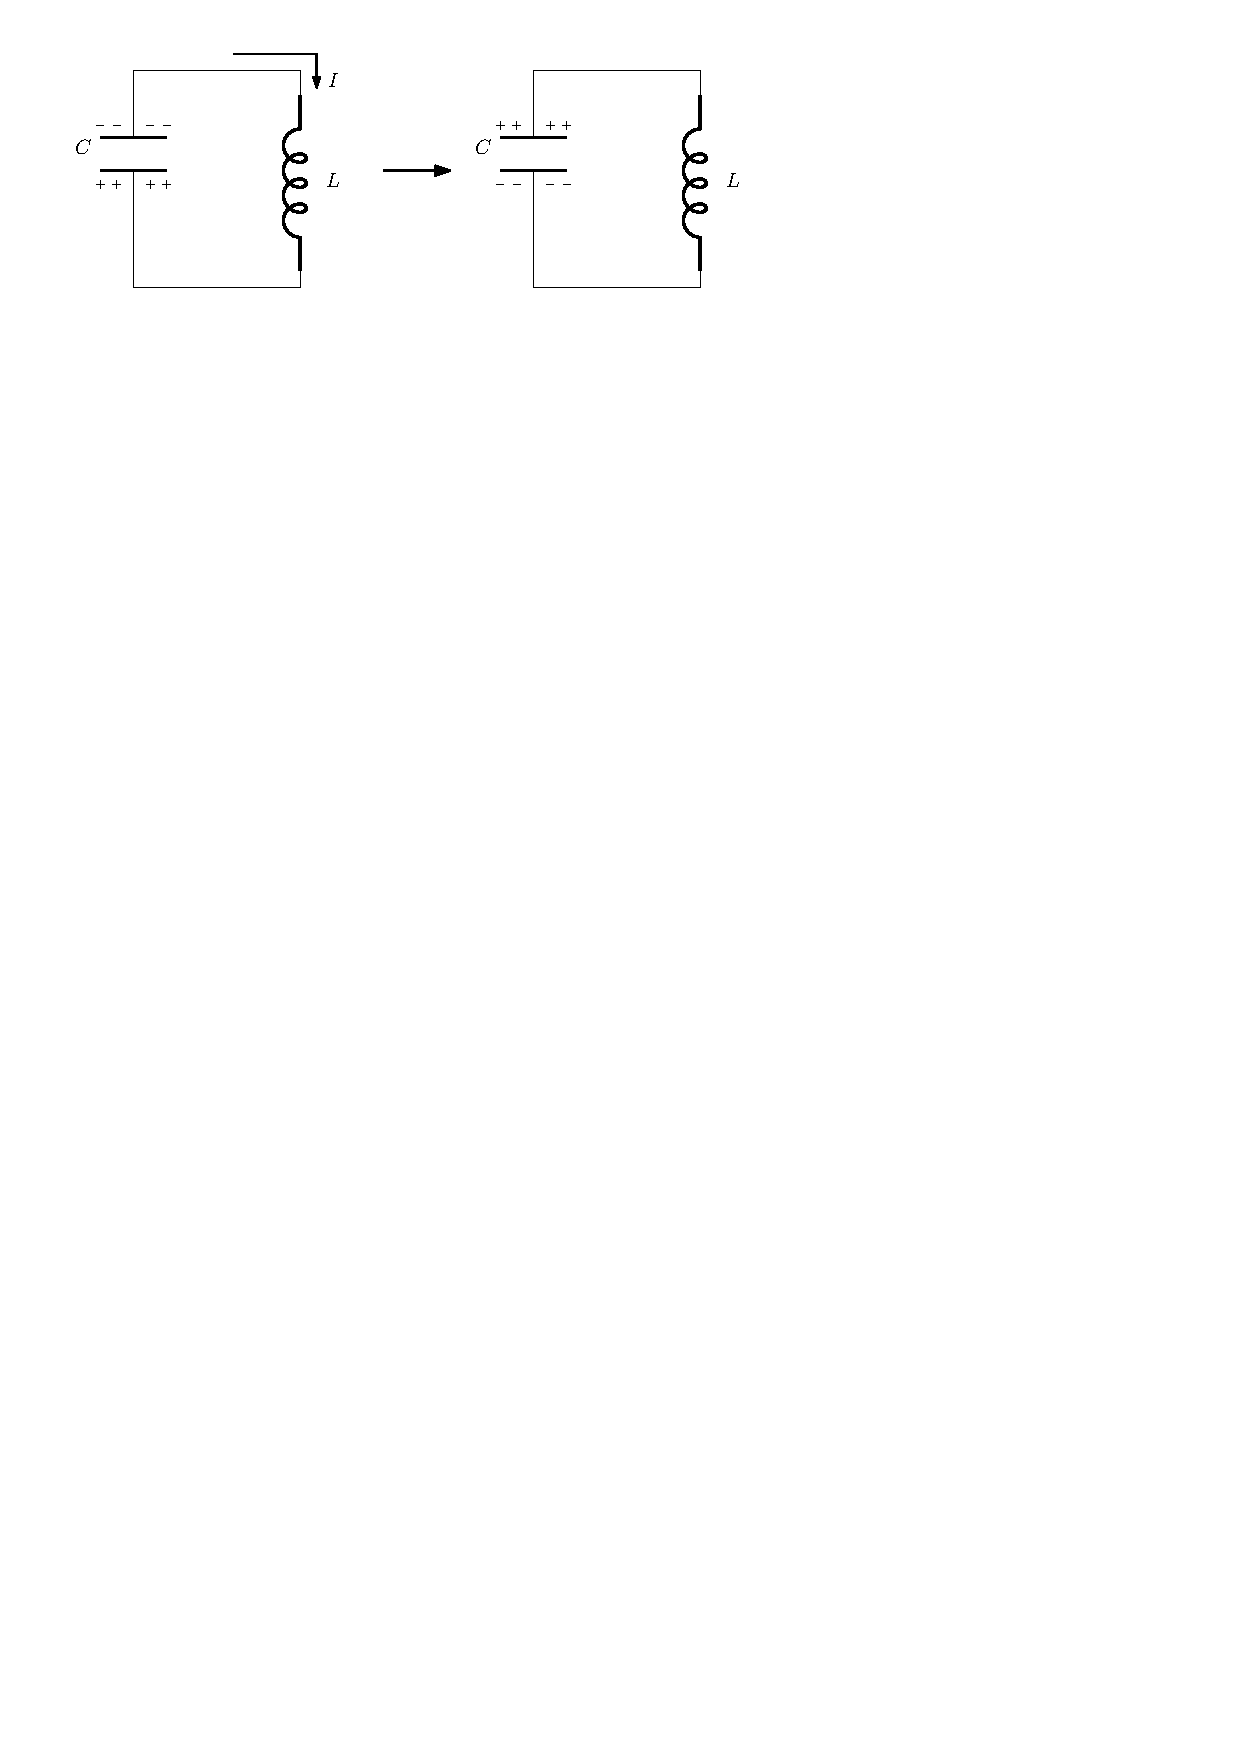
\includegraphics{figures/inductor2.pdf}
          \caption{How SHM is created by an inductor}
        \end{figure}
      \end{itemize}
\end{document}